\documentclass[12pt,a4paper,oneside]{report}

% Page dimensions and exact 2-inch margins as prescribed by college guidelines
\usepackage[a4paper,left=2in,right=2in,top=2in,bottom=2in]{geometry}
\usepackage[utf8]{inputenc}
\usepackage[T1]{fontenc}
\usepackage{mathptmx} % Times New Roman typography throughout
\usepackage{setspace}
\usepackage{titlesec}
\usepackage{tocloft}
\usepackage{graphicx}
\usepackage{booktabs}
\usepackage{longtable}
\usepackage{array}
\usepackage{multirow}
\usepackage{tabularx}
\usepackage{amsmath,amssymb}
\usepackage{listings}
\usepackage{xcolor}
\usepackage{fancyhdr}
\usepackage{caption}
\usepackage{enumitem}
\usepackage{float}
\usepackage{tikz}
\usetikzlibrary{arrows.meta,positioning,shapes.geometric,fit,calc}
\usepackage[hidelinks]{hyperref}
\usepackage{url}
\usepackage{cite}

% Typography and spacing
\onehalfspacing
\setlength{\parindent}{0.35in}
\setlength{\parskip}{4pt}

% Page numbering and running headers/footers
\pagestyle{fancy}
\fancyhf{}
\fancyfoot[C]{\thepage}
\renewcommand{\headrulewidth}{0pt}
\renewcommand{\footrulewidth}{0pt}

\fancypagestyle{plain}{
  \fancyhf{}
  \fancyfoot[C]{\thepage}
  \renewcommand{\headrulewidth}{0pt}
  \renewcommand{\footrulewidth}{0pt}
}

% Heading formatting
\titleformat{\chapter}[display]
  {\normalfont\bfseries\centering}
  {\vspace*{10mm}\normalsize CHAPTER \thechapter}
  {4pt}
  {\normalsize\MakeUppercase}
\titlespacing*{\chapter}{0pt}{0pt}{20pt}

\titleformat{\section}
  {\normalfont\normalsize\bfseries}
  {\thesection}{1em}{\MakeUppercase}

\titleformat{\subsection}
  {\normalfont\normalsize\bfseries}
  {\thesubsection}{1em}{\MakeUppercase}

\titleformat{\subsubsection}
  {\normalfont\normalsize\bfseries}
  {\thesubsubsection}{1em}{}

\titlespacing*{\section}{0pt}{12pt}{4pt}
\titlespacing*{\subsection}{0pt}{10pt}{3pt}
\titlespacing*{\subsubsection}{0pt}{8pt}{2pt}

% Code listing configuration
\definecolor{codebg}{RGB}{248,249,250}
\definecolor{codeframe}{RGB}{210,215,220}
\definecolor{codegreen}{RGB}{0,128,0}
\definecolor{codegray}{RGB}{100,100,100}
\definecolor{codepurple}{RGB}{128,0,128}

\lstdefinestyle{academiccode}{
  backgroundcolor=\color{codebg},
  basicstyle=\ttfamily\footnotesize\singlespacing,
  breakatwhitespace=false,
  breaklines=true,
  captionpos=b,
  frame=single,
  rulecolor=\color{codeframe},
  numbers=left,
  numberstyle=\tiny\color{codegray},
  numbersep=5pt,
  tabsize=2,
  showstringspaces=false,
  commentstyle=\color{codegreen},
  keywordstyle=\bfseries\color{blue},
  stringstyle=\color{codepurple}
}
\lstset{style=academiccode}

\captionsetup{font={small,singlespacing},labelfont=bf,justification=centering}
\setlength{\cftbeforechapskip}{6pt}
\setlength{\cftbeforesecskip}{3pt}

\begin{document}

% =========================================================================
% COVER / TITLE PAGE
% =========================================================================
\begin{titlepage}
\centering
\begin{singlespace}
\vspace*{0.2in}
{\bfseries\large A MINI PROJECT REPORT}\\[0.15in]
{\large ON}\\[0.2in]
{\bfseries\Large REPOSYS -- REPROGRAPHY AUTOMATION SYSTEM}\\[0.3in]
{\normalsize Submitted by}\\[0.1in]
{\bfseries\large JEFRI JIJI}\\
{\normalsize (Register Number: MGP22NMC034)}\\[0.08in]
{\normalsize Under the Project Team 04 with}\\[0.05in]
{\normalsize JERIN SEBASTIAN (MGP22NMC037)}\\
{\normalsize SETHULAKSHMI P.S (MGP22NMC050)}\\[0.25in]
{\normalsize to the}\\[0.08in]
{\bfseries\large APJ ABDUL KALAM TECHNOLOGICAL UNIVERSITY}\\[0.12in]
{\normalsize in partial fulfilment of the requirements for the award of the degree of}\\[0.1in]
{\bfseries\large MASTER OF COMPUTER APPLICATIONS}\\[0.06in]
{\bfseries\normalsize (INTEGRATED)}\\[0.25in]
\begin{figure}[H]
\centering

\includegraphics[width=1.8in,keepaspectratio]{figures/college_logo.png}
\end{figure}
\vspace{0.1in}
{\bfseries\normalsize DEPARTMENT OF COMPUTER APPLICATIONS}\\[0.06in]
{\bfseries\large SAINTGITS COLLEGE OF ENGINEERING}\\[0.04in]
{\bfseries\normalsize (AUTONOMOUS)}\\[0.04in]
{\normalsize KOTTAYAM, KERALA -- 686532}\\[0.15in]
{\normalsize OCTOBER 2026}
\end{singlespace}
\end{titlepage}

% =========================================================================
% PRELIMINARY NUMBERING
% =========================================================================
\pagenumbering{roman}
\setcounter{page}{2}

% =========================================================================
% BONAFIDE CERTIFICATE
% =========================================================================
\chapter*{BONAFIDE CERTIFICATE}
\addcontentsline{toc}{chapter}{BONAFIDE CERTIFICATE}
\begin{doublespace}
Certified that this mini project report entitled \textbf{``REPOSYS -- REPROGRAPHY AUTOMATION SYSTEM''} is a bonafide record of the work carried out by \textbf{JEFRI JIJI} (Register Number: \textbf{MGP22NMC034}) in partial fulfilment of the requirements for the award of the degree of \textbf{Master of Computer Applications (Integrated)} of APJ Abdul Kalam Technological University under our guidance and supervision during the academic year 2026. This report has not been submitted, in whole or in part, for the award of any other degree or diploma to any university or institution.
\end{doublespace}

\vspace{1.2in}
\begin{singlespace}
\noindent
\begin{tabular*}{\textwidth}{@{\extracolsep{\fill}}cc}
\textbf{[GUIDE NAME]} & \textbf{[COORDINATOR NAME]} \\
Project Guide & Project Coordinator \\
Department of Computer Applications & Department of Computer Applications \\
Saintgits College of Engineering & Saintgits College of Engineering \\[1.1in]
\textbf{[HOD NAME]} & \textbf{[PRINCIPAL NAME]} \\
Head of the Department & Principal \\
Department of Computer Applications & Saintgits College of Engineering \\
Saintgits College of Engineering & (Autonomous), Kottayam \\
\end{tabular*}
\end{singlespace}

\clearpage

% =========================================================================
% ACKNOWLEDGEMENT
% =========================================================================
\chapter*{ACKNOWLEDGEMENT}
\addcontentsline{toc}{chapter}{ACKNOWLEDGEMENT}
\begin{doublespace}
First and foremost, I offer my humble gratitude to Almighty God for showering His divine blessings and wisdom, which guided me through each stage of this project development and report writing.

I express my profound gratitude to the Management of \textbf{Saintgits College of Engineering (Autonomous)}, Kottayam, for providing excellent academic infrastructure, modern laboratory resources, and a supportive learning atmosphere conducive to technological exploration.

I place on record my sincere thanks to our respected Principal, \textbf{[PRINCIPAL NAME]}, for his leadership, encouragement, and institutional backing throughout our Integrated MCA programme.

I express my deepest appreciation to \textbf{[HOD NAME]}, Head of the Department of Computer Applications, for his visionary guidance, constructive feedback, and continuous motivation during the conceptualisation and execution of this work.

I am immensely indebted to our Project Coordinator, \textbf{[COORDINATOR NAME]}, for meticulously planning the academic reviews, providing structured schedules, and ensuring high engineering benchmarks at every milestone.

I extend my heartfelt gratitude to my Project Guide, \textbf{[GUIDE NAME]}, whose patient supervision, invaluable technical insights, and rigorous evaluation played a pivotal role in refining both the architecture of REPOSYS and this documentation.

I also extend my sincere thanks to all faculty members, technical staff, and reprography operators of the institution whose daily workflows and practical feedback shaped the functional specifications of this system.

Finally, I express my warmest thanks to my project teammates Jerin Sebastian and Sethulakshmi P.S, my classmates, and my beloved parents and family members whose unwavering moral support and encouragement enabled the successful completion of this endeavor.
\end{doublespace}

\clearpage

% =========================================================================
% ABSTRACT
% =========================================================================
\chapter*{ABSTRACT}
\addcontentsline{toc}{chapter}{ABSTRACT}
Academic reprography centres in higher education institutions serve hundreds of students, faculty, and administrative staff daily. Despite advances in campus digitisation, reprography operations have historically remained manual, paper-reliant, and inefficient. Users encounter severe physical queue congestion, privacy vulnerabilities caused by sharing confidential academic documents across personal WhatsApp channels, transaction friction due to exact cash change requirements, and lack of visibility into print job progression. Conversely, reprography counter operators face chaotic order queues, untracked paper waste from abandoned printouts, and inaccurate manual billing.

\textbf{REPOSYS (Reprography Automation System)} is an enterprise-grade, cloud-enabled web platform and hardware-integrated automation ecosystem designed to digitise the end-to-end reprography lifecycle. Architected using the modern MERN stack (MongoDB, Express.js, React 19, Node.js), REPOSYS introduces a three-tier role-based operational framework serving Students, Faculty, Counter Staff, Administrators, and Guests. The system incorporates an automated document analysis pipeline featuring client-side and server-side MIME-type validation, page-count extraction, and luminance-based blank-page detection. 

A central innovation of REPOSYS is its \textbf{Composite Priority Queue Algorithm with Dynamic Aging Deduction}. To prevent student starvation while respecting academic hierarchy, the scheduling engine calculates effective priority by combining role weights, job complexity, and an automated aging deduction function that systematically elevates long-waiting orders. Transactions are managed through integrated online Razorpay gateways, an internal digital wallet backed by MongoDB ACID transactions, and a Pay at Counter (PAC) workflow with automated timeout safeguards. Physical printing is bridged via a dedicated \textbf{Electron-based Windows Print Agent} that connects local hardware to cloud dispatchers using bi-directional Socket.IO pipelines.

Progressive Web App (PWA) capabilities enable offline queue status caching and Web Push alerts. Comprehensive quality assurance using an automated Selenium WebDriver test suite confirmed 114 passing test suites out of 120 rigorous operational cases (95.0\% passing rate). REPOSYS replaces chaotic counter queues with an auditable, cashless, transparent, and eco-friendly digital campus infrastructure.

\clearpage

% =========================================================================
% TABLE OF CONTENTS & LISTS
% =========================================================================
\tableofcontents
\clearpage
\listoftables
\clearpage
\listoffigures
\clearpage

% =========================================================================
% CHAPTER 1: INTRODUCTION
% =========================================================================
\clearpage
\pagenumbering{arabic}
\setcounter{page}{1}

\chapter{INTRODUCTION}

\section{1.1 INTRODUCTION}
In contemporary tertiary educational institutions, academic reprography and document management centres represent indispensable utility hubs. Every working day, students, research scholars, teaching faculty, and administrative personnel generate substantial demands for printing lecture notes, laboratory observation manuals, seminar presentations, dissertations, project documentation, question papers, and institutional circulars. Despite rapid campus digitisation across learning management systems (LMS) and enterprise resource planning (ERP) portals, the reprography service tier has remained an acute operational bottleneck, heavily entrenched in legacy manual practices.

In the conventional manual operating model, students are required to physically travel to the campus reprography centre, often enduring long queues during morning peak hours and pre-examination submission deadlines. Submitting electronic files frequently relies on unstandardised, insecure workarounds: students either transfer documents using uninspected USB flash drives---introducing significant malware vectors into counter workstations---or transmit files over consumer messaging platforms such as WhatsApp or Telegram. These manual practices give rise to critical vulnerabilities:
\begin{enumerate}[leftmargin=0.35in, itemsep=2pt]
  \item \textbf{Privacy Infringement and Data Exposure:} Submitting personal assignment files, identity cards, or research papers over personal mobile messaging channels exposes phone numbers and personal documents to counter staff and third-party chat databases without institutional access auditing.
  \item \textbf{Physical Counter Congestion:} Students must remain physically co-located at the reprography counter throughout the entire processing duration---from file retrieval and configuration to printing, binding, and billing---resulting in lobby overcrowding and lost instructional time.
  \item \textbf{Transaction and Billing Inefficiencies:} Cash-based counter transactions encounter persistent friction due to shortages of low-denomination physical currency notes and coins. Manual calculation of complex multi-page, double-sided, and binding combinations frequently results in billing inaccuracies and revenue leakage.
  \item \textbf{Paper Waste and Abandoned Output:} Due to communication disconnects, print operators frequently print jobs that users subsequently fail to collect, or produce incorrect orientations and color modes, leading to high volumes of abandoned paper waste and unrecoverable toner expenditure.
  \item \textbf{Absence of Prioritisation for Academic Emergencies:} Urgent examination-related printing requisitions from academic faculty are subjected to identical physical First-In, First-Out (FIFO) queue bottlenecks alongside routine student printouts, compromising institutional timeliness.
\end{enumerate}

To decisively resolve these systemic challenges, \textbf{REPOSYS (Reprography Automation System)} was conceptualised, designed, and implemented as a comprehensive, cloud-native web platform and hardware-interfaced automation ecosystem. Developed as an Integrated Master of Computer Applications (IMCA) capstone initiative at Saintgits College of Engineering (Autonomous), REPOSYS bridges academic document creators, reprography staff, institutional administrators, and physical printing machinery through an auditable, cashless, and highly responsive operational framework.

REPOSYS leverages modern software engineering standards, employing a three-tier role-based operational architecture built on the MongoDB, Express.js, React 19, and Node.js (MERN) stack. It incorporates cloud object storage via Cloudinary, secure cryptographic transaction validation with Razorpay and internal digital wallets, bi-directional event distribution via Socket.IO, an automated Progressive Web App (PWA) client, and an autonomous desktop Print Agent communicating with Windows spooler sub-systems.

\section{1.2 OBJECTIVES OF THE PROJECT}
The overarching mission of REPOSYS is to replace error-prone, manual campus document handling with a modern, dependable, and user-centric digital reprography platform. To realise this vision, the engineering objectives are classified across four functional domains:

\subsection{1.2.1 Operational and Workflow Objectives}
\begin{enumerate}[leftmargin=0.35in, itemsep=2pt]
  \item \textbf{Decoupled Document Submission:} To enable authenticated campus users and temporary kiosk guests to upload documents remotely from any browser, smartphone, or terminal, eliminating physical presence during job queuing.
  \item \textbf{Automated Document Analysis and Pre-flight Inspection:} To implement automated server-side file analysis that extracts page counts, detects color profiles, validates MIME signatures, and identifies blank pages prior to job confirmation, eliminating user error and incorrect billing.
  \item \textbf{Dynamic Priority Queue Scheduling:} To establish an equitable, multi-factor priority queue engine that balances urgent faculty requirements against student fairness through an automated aging deduction algorithm, preventing job starvation.
  \item \textbf{Secure Two-Factor Physical Handover:} To implement One-Time Password (OTP) verification and QR-based collection mechanisms at the counter, ensuring that documents are delivered exclusively to authorised owners.
\end{enumerate}

\subsection{1.2.2 Financial and Transactional Objectives}
\begin{enumerate}[leftmargin=0.35in, itemsep=2pt]
  \item \textbf{Unified Multi-Modal Payments:} To support online UPI/Card transactions via Razorpay, an internal pre-funded student digital wallet with ACID guarantees, and regulated Pay at Counter (PAC) cash workflows.
  \item \textbf{Collaborative Cost Sharing:} To provide an integrated split-payment mechanism enabling group members to disburse printing costs for shared academic projects atomically across individual student wallets.
  \item \textbf{Automated Financial Ledgering and Auditing:} To maintain an immutable, append-only transaction ledger and exportable financial reports for institutional administrative reconciliation.
\end{enumerate}

\subsection{1.2.3 Hardware and Architectural Integration Objectives}
\begin{enumerate}[leftmargin=0.35in, itemsep=2pt]
  \item \textbf{Autonomous Physical Spooling via Print Agent:} To bridge cloud backend dispatchers with local counter hardware through a specialised Electron-based Windows Print Agent that automates driver selection and document spooling.
  \item \textbf{Real-Time Operational Transparency:} To broadcast bi-directional lifecycle events (e.g., job placement, printing progress, completion notifications, queue wait-time adjustments) to connected clients without browser polling.
  \item \textbf{Automated Shop Scheduling:} To run background cron services enforcing campus operational hours (9:00 AM to 5:00 PM IST) while managing payment timeouts and uncollected order archival.
\end{enumerate}

\subsection{1.2.4 Sustainability and Security Objectives}
\begin{enumerate}[leftmargin=0.35in, itemsep=2pt]
  \item \textbf{Resource Conservation and Green Computing:} To reduce paper and toner wastage through pre-print configuration summaries, blank-page warnings, and optimized double-sided layout incentives.
  \item \textbf{End-to-End Cryptographic Security:} To enforce strict role-based access control (RBAC), JSON Web Token (JWT) session security, Cloudinary signed URL access, and data protection against unauthorized document disclosures.
\end{enumerate}

\section{1.3 SCOPE AND AVAILABILITY}
The operational scope of REPOSYS encompasses all primary document processing, queue organisation, financial settlement, physical printing, and administrative reporting requirements of an academic campus.

\subsection{1.3.1 User Roles and Stakeholder Scope}
The system establishes clearly demarcated functional boundaries for five distinct user personas:
\begin{enumerate}[leftmargin=0.35in, itemsep=2pt]
  \item \textbf{Student Persona:} Access to multi-document upload wizards, real-time cost estimation, wallet balance management, friend lists, split billing, live queue tracking, complaint lodgement, and PDF receipt downloads.
  \item \textbf{Faculty Persona:} Priority submission channels for academic and examination materials, customized delivery notes, departmental billing allocation, and direct counter priority.
  \item \textbf{Counter Staff Persona:} Operational terminal displaying active priority queues, manual cash collection controls, physical print dispatch triggers, stock inventory updates, and OTP-based pickup validation.
  \item \textbf{Administrator Persona:} Institutional oversight including dynamic price-per-page configuration, user account activation/restriction, system configuration, audit log inspection, and aggregate financial reporting.
  \item \textbf{Guest / Kiosk Persona:} Frictionless, registration-free terminal access via time-bound guest tokens and QR code tracking, with automated session expiration for campus visitors and parents.
\end{enumerate}

\subsection{1.3.2 Physical and Hardware Scope}
REPOSYS is designed to interface with standard multi-function commercial printers (MFPs), heavy-duty laser printers, and comb/spiral binding stations installed within the institutional reprography facility. Network connectivity encompasses the campus local area network (LAN), Wi-Fi, and public Internet access for remote student submissions.

\subsection{1.3.3 Operational Availability and Scheduling Boundaries}
The operational envelope of REPOSYS is governed by an automated scheduling sub-system aligned with institutional working rules:
\begin{enumerate}[leftmargin=0.35in, itemsep=2pt]
  \item \textbf{Core Operating Hours:} The reprography service automatically opens at 09:00 IST and closes at 17:00 IST, Monday through Saturday. An internal scheduler running at one-minute cron intervals evaluates Indian Standard Time (UTC+05:30) and synchronises the operational state across all active client interfaces.
  \item \textbf{Sunday and Holiday Closures:} The scheduler automatically prevents new order placement on Sundays (\texttt{day === 0}) and scheduled institutional holidays, while allowing counter staff to finish existing in-flight jobs.
  \item \textbf{Administrative Overrides:} Administrators maintain explicit supervisory privilege to trigger ``Force Open'' or ``Force Close'' modes during unscheduled maintenance, special academic workshops, or counter emergencies.
  \item \textbf{PWA Offline Availability:} When internet connectivity is temporarily interrupted, the Progressive Web App service worker provides cached access to previously retrieved order statuses and historical receipts.
\end{enumerate}

% =========================================================================
% CHAPTER 2: REQUIREMENTS AND ANALYSIS
% =========================================================================
\chapter{REQUIREMENTS AND ANALYSIS}

\section{2.1 EXISTING SYSTEM / PROBLEM STATEMENT}
To formulate a technically sound software solution, a comprehensive field analysis of the prevailing reprography system at Saintgits College of Engineering and comparable tertiary educational campuses was undertaken. The investigation revealed that document printing, duplication, and finishing services rely heavily on manual, disorganised procedures.

Figure 2.1 illustrates the operational bottlenecks and structural inefficiencies characteristic of the legacy manual workflow.

\begin{figure}[H]
\centering
\begin{tikzpicture}[node distance=1.2cm, auto,
  block/.style={rectangle, draw, fill=blue!5, text width=2.8in, text centered, rounded corners, minimum height=0.45in, font=\small},
  line/.style={draw, -{Latex[length=2.5mm]}, thick}]
  \node [block] (step1) {1. Student arrives at counter and waits in physical queue};
  \node [block, below of=step1] (step2) {2. File transferred via USB drive or personal WhatsApp};
  \node [block, below of=step2] (step3) {3. Operator opens file, checks pages, calculates price manually};
  \node [block, below of=step3] (step4) {4. Student makes cash payment (change shortage issues)};
  \node [block, below of=step4] (step5) {5. Operator manually triggers print job on local computer};
  \node [block, below of=step5] (step6) {6. Student waits at lobby until output is sorted and handed over};
  \path [line] (step1) -- (step2);
  \path [line] (step2) -- (step3);
  \path [line] (step3) -- (step4);
  \path [line] (step4) -- (step5);
  \path [line] (step5) -- (step6);
\end{tikzpicture}
\caption{Process Flow and Bottlenecks of the Existing Manual System}
\label{fig:existing_flow}
\end{figure}

The principal deficiencies and operational failure modes identified in the existing system are categorised as follows:
\begin{enumerate}[leftmargin=0.35in, itemsep=2pt]
  \item \textbf{High Latency and Lost Academic Hours:} During peak academic submission periods (continuous assessment tests, end-semester project reviews), physical queues exceed 30--40 students. Each transaction requires approximately 4 to 8 minutes of counter negotiation, consuming substantial student study time and creating severe lobby congestion.
  \item \textbf{Endpoint Security Risks and Malware Propagation:} The indiscriminate insertion of unverified USB flash drives into counter workstations exposes campus IT infrastructure to autorun trojans, ransomware, and virus infections, frequently causing workstation operating system crashes.
  \item \textbf{Privacy Breaches and Unregulated Data Sprawl:} When students share documents via personal WhatsApp numbers, their phone numbers, profile images, and private academic submissions remain stored in unmanaged personal mobile device caches and chat histories without deletion policies.
  \item \textbf{Financial Leakage and Cash Reconciliation Disputes:} Counter operators manually tally page counts across mixed single-sided, double-sided, color, and monochrome ranges. In the rush of peak hours, calculation errors occur frequently. Furthermore, lack of exact currency change creates disputes and delays.
  \item \textbf{Paper and Consumable Wastage:} Due to miscommunication regarding page ranges, color expectations, or paper orientations, unintended prints are frequently produced. Moreover, students occasionally abandon prints due to extensive wait times, resulting in uncollected paper that represents total financial and ecological loss.
  \item \textbf{Complete Lack of Operational Visibility:} Students have no mechanism to determine counter queue length, machine operational status, or estimated turnaround times before traveling to the physical facility.
\end{enumerate}

\section{2.2 PROPOSED SYSTEM / SOLUTION OVERVIEW}
\textbf{REPOSYS} resolves these systemic problems by introducing a centralised, cloud-connected digital reprography platform that decouples job submission from physical collection.

Table 2.1 summarizes the architectural and operational contrast between the existing manual process and the proposed REPOSYS solution.

\begin{table}[H]
\centering
\small
\begin{tabularx}{\textwidth}{|p{1.3in}|X|X|}
\hline
\textbf{Feature Dimension} & \textbf{Existing Manual System} & \textbf{Proposed REPOSYS} \\ \hline
\textbf{Job Submission} & Physical presence; USB drives or WhatsApp sharing & Remote web/PWA upload with pre-flight file validation \\ \hline
\textbf{Cost Calculation} & Manual operator estimation; prone to human error & Real-time algorithmic calculation with dynamic discounts \\ \hline
\textbf{Payment Methods} & Strictly physical cash; change shortages & Razorpay UPI/Cards, internal student digital wallet, regulated PAC \\ \hline
\textbf{Queue Mechanism} & Physical, unmonitored FIFO queue & Composite priority queue with dynamic anti-starvation aging \\ \hline
\textbf{Hardware Bridge} & Manual operator file opening and printer dialogs & Autonomous Electron Print Agent with background spooling \\ \hline
\textbf{Handover Security} & Open counter pickup; prone to misplacement & Two-factor OTP and QR-code collection verification \\ \hline
\textbf{Operating Hours} & Ad-hoc counter opening; unpredictable closures & Automated IST cron scheduler with real-time UI banners \\ \hline
\textbf{Audit and Logs} & Paper registers or absent record-keeping & Append-only MongoDB activity logs and automated analytics \\ \hline
\end{tabularx}
\caption{System Comparison: Existing Manual System vs. Proposed REPOSYS}
\label{tab:comparison}
\end{table}

The proposed system enforces an asynchronous, transparent document workflow:
\begin{enumerate}[leftmargin=0.35in, itemsep=2pt]
  \item \textbf{Remote Multi-Document Upload:} Users upload PDF, Word, or image documents from mobile or desktop browsers. The backend extracts structural metadata, counts pages, and performs blank-page detection.
  \item \textbf{Transparent Algorithmic Pricing:} The user customises printing parameters (color mode, copies, duplexing, binding, paper size) and receives a deterministic price quotation calculated from admin-configured rates.
  \item \textbf{Frictionless Settlement:} The user completes payment using Razorpay, wallet balance, or cash at counter, triggering immediate queue assignment.
  \item \textbf{Dynamic Priority Queue Placement:} The order enters the processing queue with an effective priority score combining role priority, complexity, and wait-time aging.
  \item \textbf{Automated Spooling and Production:} The counter staff or automated Print Agent spools the validated job to the assigned physical printer.
  \item \textbf{Secure Handover via OTP:} Upon completion, the customer receives a pickup alert and presents a 4-digit OTP or QR code to claim the output.
\end{enumerate}

\section{2.3 FEASIBILITY STUDY}
Before commencing technical development, a comprehensive feasibility study was conducted to evaluate the viability of REPOSYS across four key engineering dimensions.

\subsection{2.3.1 Technical Feasibility}
The technical feasibility evaluates whether the available hardware, software stacks, and cloud infrastructure can support the target system requirements:
\begin{itemize}[leftmargin=0.35in, itemsep=2pt]
  \item \textbf{Technology Stack Maturity:} The MERN stack (MongoDB, Express.js, React 19, Node.js) represents an industry-standard, battle-tested software architecture. Node.js provides non-blocking, asynchronous I/O ideal for handling concurrent upload streams and WebSocket events.
  \item \textbf{Cloud Storage and Processing:} Cloudinary provides reliable cloud object storage with signed secure URLs, while client-side \texttt{pdfjs-dist} and server-side \texttt{pdf-lib} provide robust programmatic document parsing.
  \item \textbf{Real-Time Communication:} Socket.IO enables low-latency, full-duplex bi-directional communication between connected clients, staff dashboards, and print agents without consuming excessive server memory.
  \item \textbf{Hardware Interfacing via Electron:} The Electron framework provides direct access to Windows operating system APIs and the local print spooler (\texttt{pdf-to-printer}), allowing the desktop Print Agent to control physical hardware seamlessly.
\end{itemize}
The technical architecture requires no proprietary, untried technology; all components have mature documentation, strong community support, and verified open-source libraries. Hence, the project is technically feasible.

\subsection{2.3.2 Operational Feasibility}
Operational feasibility assesses how effectively the proposed solution integrates into the daily routines of campus stakeholders:
\begin{itemize}[leftmargin=0.35in, itemsep=2pt]
  \item \textbf{Student and Faculty Usability:} Students and faculty already use smartphones and web browsers daily. The intuitive 3-step ordering wizard, mobile-responsive layout, and PWA installation require zero formal user training.
  \item \textbf{Counter Staff Ergonomics:} Counter operators transition from manual file handling and cash calculation to an intuitive dashboard that displays incoming jobs, automatically computes totals, and verifies handovers via single-click OTP entry.
  \item \textbf{Institutional Governance:} Administrators receive real-time visibility into machine status, paper consumption, daily revenue, and staff incident reports, substantially easing operational auditing.
\end{itemize}
Because REPOSYS directly eliminates manual bottlenecks without imposing complicated new workflows, user acceptance is exceptionally high. Therefore, the system is operationally feasible.

\subsection{2.3.3 Economic Feasibility}
Economic feasibility weighs the development, deployment, and operational expenditures against the tangible and intangible cost savings:
\begin{itemize}[leftmargin=0.35in, itemsep=2pt]
  \item \textbf{Development Cost:} The platform is constructed entirely using open-source frameworks (React, Node.js, Express, MongoDB Community/Atlas free tier, Vite, Tailwind CSS, Electron), incurring zero proprietary software licensing fees.
  \item \textbf{Hosting and Cloud Infrastructure:} Cloud hosting on scalable platforms (Vercel for frontend, Render for backend, MongoDB Atlas M0/M10 for database) provides cost-effective hosting tailored to campus traffic profiles.
  \item \textbf{Resource Savings:} Eliminating uncollected prints and wasted paper saves hundreds of sheets per week. Accurate automated billing prevents revenue leakage.
  \item \textbf{Productivity Dividends:} Minimising queue wait times recovers valuable instructional and research hours for students and faculty.
\end{itemize}
The projected operational savings and efficiency gains substantially outweigh the negligible deployment costs, confirming high economic feasibility.

\subsection{2.3.4 Schedule Feasibility}
The capstone project was structured across a 17-week academic timeline prescribed by the Department of Computer Applications for course \textbf{20IMCAP501 (Mini Project - 2)}. The schedule allotted realistic durations for requirements analysis, system architecture, database design, backend coding, frontend development, payment/agent integration, and automated testing. Table 2.2 in Section 2.5 confirms that all deliverables aligned with institutional assessment milestones.

\section{2.4 CONCEPTUAL MODELLING}
Conceptual modelling captures the high-level boundaries, external entities, and data flows governing REPOSYS.

\subsection{2.4.1 Level 0 Context Data Flow Diagram}
The Level 0 Context DFD depicts REPOSYS as a centralised system interacting with five primary external entities: Students/Faculty, Counter Staff, Administrators, Razorpay Payment Gateway, and Cloudinary Storage.

\begin{figure}[H]
\centering
\begin{tikzpicture}[node distance=1.8cm, auto,
  process/.style={circle, draw=blue!80, fill=blue!10, thick, text width=1.1in, text centered, font=\bfseries\small},
  entity/.style={rectangle, draw=black!80, fill=gray!10, thick, text width=1.1in, text centered, rounded corners, minimum height=0.35in, font=\small},
  line/.style={draw, -{Latex[length=2mm]}, thick}]
  
  \node [process] (system) {0.0\\REPOSYS Platform};
  \node [entity, above of=system, yshift=0.8cm] (user) {Students / Faculty};
  \node [entity, right of=system, xshift=1.6cm] (staff) {Counter Staff};
  \node [entity, below of=system, yshift=-0.8cm] (admin) {Administrator};
  \node [entity, left of=system, xshift=-1.6cm] (gateway) {Payment Gateway (Razorpay)};
  
  \path [line] (user) -- node[left, font=\tiny]{Uploads, Orders} (system);
  \path [line] (system) -- node[right, font=\tiny]{Receipts, OTPs} (user);
  \path [line] (system) -- node[above, font=\tiny]{Queue, Jobs} (staff);
  \path [line] (staff) -- node[below, font=\tiny]{OTP, Cash Status} (system);
  \path [line] (admin) -- node[right, font=\tiny]{Pricing, Config} (system);
  \path [line] (system) -- node[left, font=\tiny]{Analytics, Logs} (admin);
  \path [line] (system) -- node[above, font=\tiny]{Payment Requisition} (gateway);
  \path [line] (gateway) -- node[below, font=\tiny]{Signature / Status} (system);
\end{tikzpicture}
\caption{Level 0 Context Data Flow Diagram of REPOSYS}
\label{fig:dfd_level0}
\end{figure}

\subsection{2.4.2 Level 1 Functional Data Flow Diagram}
The Level 1 DFD decomposes REPOSYS into its major functional processes: Authentication (1.0), Document Upload and Inspection (2.0), Order Configuration and Costing (3.0), Payment Settlement (4.0), Queue Scheduling (5.0), and Physical Production Handover (6.0).

\begin{figure}[H]
\centering
\begin{tikzpicture}[node distance=1.3cm, auto,
  proc/.style={rectangle, draw=blue!70, fill=blue!5, rounded corners, text width=2.8in, text centered, minimum height=0.35in, font=\small},
  store/.style={rectangle, draw=black!70, fill=yellow!10, text width=2.8in, text centered, minimum height=0.28in, font=\footnotesize},
  line/.style={draw, -{Latex[length=2mm]}, thick}]
  
  \node [proc] (p1) {1.0 User Authentication \& Role Verification};
  \node [proc, below of=p1] (p2) {2.0 Document Upload, MIME Check \& Analysis};
  \node [proc, below of=p2] (p3) {3.0 Order Configuration \& Dynamic Cost Estimation};
  \node [proc, below of=p3] (p4) {4.0 Payment Processing (Wallet / Razorpay / PAC)};
  \node [proc, below of=p4] (p5) {5.0 Priority Queue Scheduling \& Aging Engine};
  \node [proc, below of=p5] (p6) {6.0 Print Dispatch, OTP Handover \& Receipting};
  
  \path [line] (p1) -- (p2);
  \path [line] (p2) -- (p3);
  \path [line] (p3) -- (p4);
  \path [line] (p4) -- (p5);
  \path [line] (p5) -- (p6);
\end{tikzpicture}
\caption{Level 1 Functional Data Flow Diagram of the Complete Order Pipeline}
\label{fig:dfd_level1}
\end{figure}

\section{2.5 PLANNING AND SCHEDULING}
The engineering development of REPOSYS was structured using the Agile Scrum methodology across a 17-week semester schedule prescribed by the official Scrum Register for course \textbf{20IMCAP501 (Mini Project - 2)}.

Table 2.2 documents the formal project schedule, task assignments, deliverables, and review milestones.

\begin{table}[H]
\centering
\small
\begin{tabularx}{\textwidth}{|p{0.55in}|p{0.95in}|X|p{0.65in}|}
\hline
\textbf{Week} & \textbf{Date Range} & \textbf{Planned Work and Key Deliverables} & \textbf{Status} \\ \hline
\textbf{W1} & 01--04 Jul 2026 & Topic selection, domain research, and approved synopsis & 100\% Done \\ \hline
\textbf{W2} & 06--10 Jul 2026 & System study, feasibility analysis, module identification & 100\% Done \\ \hline
\textbf{W3} & 13--17 Jul 2026 & Requirements gathering, user stories, UI wireframes & 100\% Done \\ \hline
\textbf{W4} & 20--22 Jul 2026 & UML modeling, ER schema normalization, Git repo setup & 100\% Done \\ \hline
\textbf{W5} & 27--29 Jul 2026 & Core structure setup, basic UI components (\textbf{Review 0}) & 100\% Done \\ \hline
\textbf{W6} & 03--07 Aug 2026 & Authentication, JWT security, user profile management & 100\% Done \\ \hline
\textbf{W7} & 10--14 Aug 2026 & Document upload pipeline, Cloudinary integration, testing & 100\% Done \\ \hline
\textbf{W8} & 17--21 Aug 2026 & Priority queue, pricing engine, 50\% evaluation (\textbf{Review 1}) & 100\% Done \\ \hline
\textbf{W9} & 01--05 Sep 2026 & Razorpay gateway, wallet atomic transactions & 100\% Done \\ \hline
\textbf{W10} & 07--11 Sep 2026 & Staff counter dashboard, OTP pickup verification & 100\% Done \\ \hline
\textbf{W11} & 14--18 Sep 2026 & Admin console, inventory tracker, Selenium suite build & 100\% Done \\ \hline
\textbf{W12} & 21--25 Sep 2026 & Socket.IO real-time engine, 80\% Scrum Master Review & 100\% Done \\ \hline
\textbf{W13} & 28--30 Sep 2026 & Electron Print Agent, shop cron scheduler, cloud hosting & 100\% Done \\ \hline
\textbf{W14} & 05--09 Oct 2026 & PWA service worker, push alerts, final bug rectification & 100\% Done \\ \hline
\textbf{W15} & 12--14 Oct 2026 & Final assessment board evaluation, live demo (\textbf{Review 2}) & 100\% Done \\ \hline
\textbf{W16} & 14 Oct 2026 & Final project report submission and print verification & 100\% Done \\ \hline
\textbf{W17} & 15 Oct 2026 & Hard-bound submission, signed Scrum register, git logs & 100\% Done \\ \hline
\end{tabularx}
\caption{Official Project Schedule and Milestone Tracking (Scrum Register 20IMCAP501)}
\label{tab:schedule}
\end{table}

% =========================================================================
% CHAPTER 3: SYSTEM SPECIFICATION
% =========================================================================
\chapter{SYSTEM SPECIFICATION}

\section{3.1 SOFTWARE AND HARDWARE REQUIREMENTS}
To guarantee reliable execution across development, testing, and production tiers, clear hardware and software operational requirements were established.

\subsection{3.1.1 Software Requirement}
Table 3.1 enumerates the complete software specifications and production dependency versions derived directly from the application's configuration manifests.

\begin{table}[H]
\centering
\small
\begin{tabularx}{\textwidth}{|p{1.2in}|p{1.3in}|X|}
\hline
\textbf{Layer / Component} & \textbf{Technology / Library} & \textbf{Version / Configuration} \\ \hline
\textbf{Server Runtime} & Node.js & v20.12.0 LTS (or higher) \\ \hline
\textbf{Backend Framework} & Express.js & v4.19.2 \\ \hline
\textbf{Database Engine} & MongoDB Atlas / Community & v7.0.x with Mongoose ODM \\ \hline
\textbf{Frontend Framework} & React.js & v19.2.4 (Vite bundler) \\ \hline
\textbf{CSS Framework} & Tailwind CSS & v4.2.2 with PostCSS \\ \hline
\textbf{Real-Time Engine} & Socket.IO & Server \& Client v4.8.3 \\ \hline
\textbf{Cloud File Storage} & Cloudinary SDK & Multer-storage-cloudinary \\ \hline
\textbf{Payment Gateway} & Razorpay Node SDK & v2.9.6 (Webhook verification) \\ \hline
\textbf{Desktop Agent} & Electron & v30.0.0 with pdf-to-printer \\ \hline
\textbf{Document Parser} & pdf-lib \& pdfjs-dist & Server-side PDF analysis \\ \hline
\textbf{Security Packages} & Helmet, bcryptjs, cors & Salt factor 12, rate limiter \\ \hline
\textbf{Scheduler} & node-cron & 5-field cron running * * * * * \\ \hline
\textbf{Testing Engine} & Selenium WebDriver & Python 3.12, pytest-html 4.2.0 \\ \hline
\textbf{Client Browsers} & Chromium, Firefox, Edge & Modern HTML5 / ES6 standards \\ \hline
\end{tabularx}
\caption{Production Software Stack and Dependency Specifications}
\label{tab:software_reqs}
\end{table}

\subsection{3.1.2 Hardware Requirement}
The system hardware requirements are divided across the production cloud server, the physical counter workstation, and the user client devices:
\begin{enumerate}[leftmargin=0.35in, itemsep=2pt]
  \item \textbf{Production Cloud Application Server:}
    \begin{itemize}[itemsep=1pt]
      \item Processor: Quad-Core 64-bit x86/ARM CPU (2.4 GHz or higher).
      \item Random Access Memory (RAM): Minimum 4 GB RAM (8 GB recommended for concurrent upload parsing).
      \item Persistent Disk: 20 GB SSD storage for operating system, temporary buffer caches, and application logs.
      \item Network Interface: 100 Mbps full-duplex uplink with high-bandwidth availability.
    \end{itemize}
  \item \textbf{Counter Staff Workstation \& Print Agent Host:}
    \begin{itemize}[itemsep=1pt]
      \item Operating System: Microsoft Windows 10 / Windows 11 (64-bit) for Windows Spooler API compatibility.
      \item Processor: Intel Core i3 / AMD Ryzen 3 or equivalent.
      \item RAM: Minimum 4 GB RAM.
      \item Disk: 10 GB free space for spooling temporary PDF documents.
      \item Peripherals: USB 3.0 / Gigabit Ethernet interface connecting local multi-function printers, thermal receipt printer, and 2D barcode / QR-code scanner.
    \end{itemize}
  \item \textbf{Student / Faculty Client Devices:}
    \begin{itemize}[itemsep=1pt]
      \item Smartphone or Laptop: Any standard Android, iOS, Windows, macOS, or Linux device equipped with an HTML5-compliant web browser.
      \item Network: 4G/5G mobile data or campus Wi-Fi connectivity.
    \end{itemize}
  \item \textbf{Target Reprography Hardware:}
    \begin{itemize}[itemsep=1pt]
      \item Networked Heavy-Duty Commercial Multifunction Printers (Canon, HP, Ricoh, Konica Minolta).
      \item Comb and Spiral document binding machine.
    \end{itemize}
\end{enumerate}

\section{3.2 FUNCTIONAL SPECIFICATIONS}
The functional capabilities of REPOSYS were architected across 39 distinct system features. The primary operational specifications are detailed below:
\begin{enumerate}[leftmargin=0.35in, itemsep=2pt]
  \item \textbf{User Authentication and Role Verification (Feature 1):} Implements secure registration with email validation, password encryption via bcrypt (12 salt rounds), and stateless JSON Web Token (JWT) session generation stored in HTTP-only secure cookies.
  \item \textbf{Composite Priority Queue Management (Feature 2):} Dynamically sorts in-flight printing jobs based on a composite score combining user role, job duration, and waiting time aging deduction.
  \item \textbf{Document Upload and Pre-Flight Inspection (Feature 3):} Supports multi-format upload (PDF, DOCX, PNG, JPEG) with client and server MIME validation, computing page count, color percentage, and blank-page alerts.
  \item \textbf{Order Configuration Wizard (Feature 4):} Multi-step wizard allowing users to configure copies, color mode (Monochrome vs. Full Color), duplexing (Single vs. Double-sided), paper size (A4, A3, Legal), and binding (Spiral, Staple, None).
  \item \textbf{Dynamic Cost Calculation Engine (Feature 7):} Deterministic price estimation applying unit rates, duplex discounts (0.85 multiplier), binding costs, and active coupon codes.
  \item \textbf{Multi-Channel Payment Settlement (Feature 8):} Real-time payment processing through Razorpay (UPI, Netbanking, Cards), internal user wallet with atomic MongoDB transactions, and cash Pay at Counter.
  \item \textbf{Order Tracking Timeline (Feature 10):} Visual status progression tracking: \texttt{Pending}, \texttt{In\_Queue}, \texttt{Processing}, \texttt{ReadyForPickup}, \texttt{Completed}, and \texttt{Cancelled}.
  \item \textbf{Counter Staff Production Dashboard (Feature 13):} Live terminal displaying queue orders, cash collection triggers, physical print dispatch, and stock status.
  \item \textbf{OTP-Protected Pickup Handover (Feature 28):} High-security order delivery requiring counter staff to enter the customer's 4-digit OTP or scan their QR token before order status changes to \texttt{Completed}.
  \item \textbf{Smart Kiosk Session Mode (Feature 36):} Registration-free guest ordering generating temporary UUID session tokens with 2-hour sliding expirations and automatic inactivity wipe.
  \item \textbf{Collaborative Friend Chat and Split Requests (Features 38 \& 39):} Peer-to-peer friend chat and collaborative group-order payment splitting with atomic multi-wallet deductions.
\end{enumerate}

\section{3.3 TOOLS AND PLATFORMS USED}
\begin{enumerate}[leftmargin=0.35in, itemsep=2pt]
  \item \textbf{React 19 with Vite:} Delivers a lightning-fast Single Page Application (SPA) leveraging React Server Components, custom hooks (\texttt{useSocket}, \texttt{useAuth}), and optimized bundle splitting via Vite.
  \item \textbf{Node.js and Express.js:} Forms the asynchronous API gateway capable of non-blocking I/O operations, routing, middleware orchestration, and streaming multipart upload data.
  \item \textbf{MongoDB Atlas and Mongoose:} Flexible document-oriented NoSQL database providing schema validation, high-speed secondary indexing, and multi-document ACID transaction guarantees.
  \item \textbf{Socket.IO:} Enterprise-grade WebSocket abstraction managing room-based event broadcasting (\texttt{queue:serviceType}, \texttt{user:userId}, \texttt{staff}, \texttt{admin}) with automatic HTTP long-polling fallback.
  \item \textbf{Cloudinary Media Cloud:} Enterprise object storage managing uploaded documents with AES-256 cloud encryption, time-delimited signed URLs, and automated PDF-to-thumbnail transformation.
  \item \textbf{Razorpay API:} RBI-compliant digital payment gateway facilitating seamless student payments across Google Pay, PhonePe, Paytm, debit/credit cards, and net banking.
  \item \textbf{Electron Framework:} Powers the desktop Print Agent, bridging web APIs to native Windows operating system commands, Windows PowerShell, and spooler utilities.
  \item \textbf{Selenium WebDriver and Pytest:} Comprehensive automated testing suite simulating end-to-end user interactions, verifying route protection, and auditing UI flows across real browser sessions.
\end{enumerate}

\section{3.4 DEVELOPMENT ENVIRONMENT}
The development lifecycle was conducted under structured development conventions:
\begin{itemize}[leftmargin=0.35in, itemsep=2pt]
  \item \textbf{Version Control Configuration:} Git and GitHub were utilised for branching, feature pull requests, and commit tracking.
  \item \textbf{Environment Variable Management:} Configuration isolation was maintained through \texttt{.env.development} and \texttt{.env.production} files, segregating API keys, MongoDB connection URIs, Razorpay secrets, and Cloudinary credentials.
  \item \textbf{Cross-Origin Resource Sharing (CORS):} Controlled through strict origin whitelisting in \texttt{origins.js}, permitting requests exclusively from authorized frontend and print-agent hosts.
  \item \textbf{Database Seeding Scripts:} Automated seeding scripts (\texttt{seedAdmin.js}, \texttt{seedInventory.js}) populated default system configurations, catalog pricing rules, paper stock, and supervisory accounts upon initialization.
\end{itemize}

% =========================================================================
% CHAPTER 4: SYSTEM DESIGN
% =========================================================================
\chapter{SYSTEM DESIGN}

\section{4.1 MODULE DESCRIPTIONS}
REPOSYS is engineered around four deeply integrated subsystem modules, each tailored to distinct operational responsibilities within the reprography ecosystem.

\subsection{4.1.1 User and Customer Module}
The User Module provides authenticated students, faculty, and campus guests with an intuitive digital storefront for document submission and lifecycle management:
\begin{enumerate}[leftmargin=0.35in, itemsep=2pt]
  \item \textbf{Authentication and Profile Subsystem:} Manages user registration, JWT login, profile editing, and password recovery via encrypted email tokens.
  \item \textbf{Three-Step Order Placement Wizard:} Guides the customer through: (i) File drag-and-drop with pre-flight analysis; (ii) Print configuration (copies, color, duplexing, paper format, binding); and (iii) Cost review and payment gateway selection.
  \item \textbf{Digital Wallet Subsystem:} Displays pre-funded balances, transaction logs, and single-click wallet debits backed by MongoDB multi-document ACID transactions.
  \item \textbf{Order Tracking and Digital Receipts:} Renders an active order timeline with live queue position updates, countdown timers, pickup OTP codes, and dynamically generated PDF receipts.
  \item \textbf{Collaborative Tools:} Manages student friend connections, direct peer messaging, and collaborative split-order requests.
\end{enumerate}

\subsection{4.1.2 Counter Staff Module}
The Counter Staff Module equips reprography operators with a dedicated operational terminal designed for high-throughput, error-free counter processing:
\begin{enumerate}[leftmargin=0.35in, itemsep=2pt]
  \item \textbf{Active Priority Queue Board:} Real-time dashboard grouping active jobs by service type (Printing, Photocopying, Scanning, Binding), sorted dynamically by effective priority score.
  \item \textbf{Production Controls:} Enables operators to trigger manual print dispatches, mark orders as \texttt{Processing}, and transition finished jobs to \texttt{ReadyForPickup}.
  \item \textbf{Cash-at-Counter Settlement:} Single-click verification for cash collections, updating \texttt{paymentStatus} from \texttt{Cash\_Pending} to \texttt{Paid} and synchronizing the daily counter register.
  \item \textbf{OTP-Protected Handover Terminal:} Requires entry of the customer's 4-digit verification code or barcode scan before finalizing delivery.
  \item \textbf{Incident Reporting Subsystem:} Enables operators to log equipment malfunctions, toner outages, or customer disputes directly to administrators.
\end{enumerate}

\subsection{4.1.3 Administrator Module}
The Administrator Module provides institutional supervisors with governance and configuration capabilities:
\begin{enumerate}[leftmargin=0.35in, itemsep=2pt]
  \item \textbf{Dynamic Tariff and Pricing Control:} Live configuration of unit costs for black-and-white, color, double-sided discounts, binding modes, and paper types without requiring server restarts.
  \item \textbf{User and Role Governance:} Supervisory oversight of student, faculty, and staff accounts, including role reassignments and account restrictions.
  \item \textbf{Consumable Inventory Tracker:} Automated monitoring of A4/A3 paper reams, toner cartridges, and binding coils with low-stock warning thresholds.
  \item \textbf{Append-Only Audit Logging:} Comprehensive activity tracking logging every sensitive administrative, financial, and operational action.
  \item \textbf{Automated Shop Operations Control:} Manual overrides for shop opening hours (\texttt{schedule}, \texttt{manual\_open}, \texttt{manual\_close}).
\end{enumerate}

\subsection{4.1.4 Print Agent Module}
The Print Agent is an autonomous Electron desktop background service deployed on counter workstations:
\begin{enumerate}[leftmargin=0.35in, itemsep=2pt]
  \item \textbf{Hardware Discovery:} Periodically executes Windows PowerShell cmdlets (\texttt{Get-Printer}) to detect installed physical print drivers and online/offline states.
  \item \textbf{Secure Cloud Job Retrieval:} Authenticates using unique agent tokens, listens for Socket.IO dispatch events, and fetches documents via temporary signed Cloudinary URLs.
  \item \textbf{Spooler Execution:} Invokes native Windows printing utilities (\texttt{pdf-to-printer}) to spool files directly into the target printer queue.
  \item \textbf{Heartbeat Telemetry:} Emits heartbeat pings every 30 seconds to update cloud registries regarding hardware readiness.
\end{enumerate}

\section{4.2 DATA / SCHEMA DESIGN}
Persistence in REPOSYS is managed through MongoDB using Mongoose Object Data Modeling (ODM). The database comprises 23 primary collections structured to support rapid lookups, transactional integrity, and comprehensive auditability.

Table 4.1 details the primary collections, indexing strategies, and schema definitions.

\begin{table}[H]
\centering
\small
\begin{tabularx}{\textwidth}{|p{1.1in}|p{1.1in}|X|}
\hline
\textbf{Collection} & \textbf{Key Indexes} & \textbf{Core Schema Fields \& Data Types} \\ \hline
\textbf{User} & \texttt{email} (unique) & \texttt{name} (String), \texttt{email} (String), \texttt{password} (Hash), \texttt{role} (Enum: Student, Faculty, Staff, Admin), \texttt{department} (String), \texttt{walletBalance} (Number), \texttt{isVerified} (Boolean). \\ \hline
\textbf{Order} & \texttt{orderNumber} (unique), \texttt{userId}, \texttt{status}, \texttt{createdAt} & \texttt{orderNumber} (String), \texttt{userId} (Ref: User), \texttt{serviceType} (Enum), \texttt{documents} (Array), \texttt{totalCost} (Number), \texttt{paymentStatus} (Enum), \texttt{status} (Enum), \texttt{priorityScore} (Number), \texttt{pickupOtp} (String), \texttt{qrCode} (String). \\ \hline
\textbf{Document} & \texttt{orderId}, \texttt{userId} & \texttt{fileName} (String), \texttt{fileUrl} (String), \texttt{fileType} (String), \texttt{pageCount} (Number), \texttt{colorPages} (Number), \texttt{blankPages} (Array), \texttt{fileSize} (Number). \\ \hline
\textbf{Payment} & \texttt{razorpayOrderId}, \texttt{orderId} & \texttt{orderId} (Ref: Order), \texttt{userId} (Ref: User), \texttt{amount} (Number), \texttt{method} (Enum: Razorpay, Wallet, Cash), \texttt{transactionId} (String), \texttt{status} (Enum: Pending, Completed, Failed). \\ \hline
\textbf{Wallet} & \texttt{userId} (unique) & \texttt{userId} (Ref: User), \texttt{balance} (Number), \texttt{currency} (String), \texttt{lastUpdated} (Date). \\ \hline
\textbf{WalletTransaction} & \texttt{walletId}, \texttt{createdAt} & \texttt{walletId} (Ref: Wallet), \texttt{type} (Enum: Credit, Debit), \texttt{amount} (Number), \texttt{description} (String), \texttt{balanceAfter} (Number). \\ \hline
\textbf{Complaint} & \texttt{orderId}, \texttt{userId}, \texttt{status} & \texttt{orderId} (Ref: Order), \texttt{userId} (Ref: User), \texttt{category} (String), \texttt{subject} (String), \texttt{description} (String), \texttt{status} (Enum: Open, In\_Progress, Resolved), \texttt{messages} (Array). \\ \hline
\textbf{InventoryItem} & \texttt{itemCode} (unique) & \texttt{itemName} (String), \texttt{category} (Enum: Paper, Toner, Binding), \texttt{quantity} (Number), \texttt{threshold} (Number), \texttt{unitCost} (Number). \\ \hline
\textbf{SystemConfig} & Singleton & \texttt{pricing} (Object), \texttt{operatingHours} (Object), \texttt{shopMode} (Enum: schedule, manual\_open, manual\_close), \texttt{isManuallyOpen} (Boolean). \\ \hline
\textbf{PrintAgentRegistry} & \texttt{agentId} (unique) & \texttt{agentId} (String), \texttt{hostName} (String), \texttt{ipAddress} (String), \texttt{status} (Enum: Online, Offline), \texttt{lastHeartbeat} (Date), \texttt{printers} (Array). \\ \hline
\end{tabularx}
\caption{Database Schema Specifications of Core REPOSYS Collections}
\label{tab:schema_specs}
\end{table}

\section{4.3 PROCEDURAL / FLOW DESIGN}

\subsection{4.3.1 Priority Queue and Aging Mathematical Model}
To balance institutional hierarchy against fair queue wait times, REPOSYS executes a dynamic priority evaluation algorithm within \texttt{queueService.js}. A lower score denotes a higher processing priority.

The base priority score ($S_{\text{base}}$) is evaluated upon order creation:
\begin{equation}
S_{\text{base}} = P_{\text{role}} + \lfloor T_{\text{est}} \rfloor
\end{equation}
where $P_{\text{role}}$ represents the categorical role priority:
\begin{equation}
P_{\text{role}} = 
\begin{cases} 
100, & \text{if User Role} = \text{Faculty} \\
150, & \text{if User Role} = \text{Staff} \\
200, & \text{if User Role} \in \{\text{Student}, \text{Guest}\}
\end{cases}
\end{equation}
and $T_{\text{est}}$ represents the estimated physical production duration in minutes.

To prevent job starvation where an influx of faculty orders permanently postpones student orders, the system recalculates the effective priority score ($S_{\text{eff}}$) dynamically:
\begin{equation}
D_{\text{aging}} = \max\left(0, \left\lfloor \frac{T_{\text{wait}} - 1}{60} \right\rfloor\right) \times 20
\end{equation}
\begin{equation}
S_{\text{eff}} = S_{\text{base}} - D_{\text{aging}}
\end{equation}
where $T_{\text{wait}}$ is the elapsed waiting time in minutes. For every full hour of counter waiting, the order's score is reduced by 20 points, steadily moving the job ahead in queue. When two orders possess equal effective scores, First-In, First-Out (\texttt{createdAt} ascending) serves as the definitive tie-breaker.

\subsection{4.3.2 Automated Shop Scheduling State Machine}
The operating availability of the reprography centre is governed by an automated scheduler in \texttt{shopScheduler.js} executing every minute via \texttt{node-cron} (\texttt{* * * * *}).

Figure 4.1 depicts the operational state machine controlling shop availability.

\begin{figure}[H]
\centering
\begin{tikzpicture}[node distance=1.4cm, auto,
  state/.style={rectangle, draw=blue!80, fill=blue!5, rounded corners, text width=2.6in, text centered, minimum height=0.4in, font=\small},
  line/.style={draw, -{Latex[length=2mm]}, thick}]
  
  \node [state] (cron) {Cron Triggered Every Minute\\(* * * * *)};
  \node [state, below of=cron] (time) {Evaluate IST Time (UTC + 05:30)\\Check: Monday--Saturday, 09:00 to 17:00};
  \node [state, below of=time] (check) {Check \texttt{shopMode} Configuration\\Mode = \texttt{schedule} (Evaluate IST)\\Mode = \texttt{manual\_open} / \texttt{manual\_close} (Override)};
  \node [state, below of=check] (emit) {Broadcast State Change via Socket.IO\\Events: \texttt{shop\_opened} or \texttt{shop\_closed}};
  
  \path [line] (cron) -- (time);
  \path [line] (time) -- (check);
  \path [line] (check) -- (emit);
\end{tikzpicture}
\caption{Automated Shop Scheduling Logic and Operational State Transitions}
\label{fig:shop_scheduler}
\end{figure}

\subsection{4.3.3 Order Expiration and Pay-at-Counter Timeout Management}
In addition to shop hours, background services in \texttt{cronJobs.js} enforce financial and operational timeouts:
\begin{itemize}[leftmargin=0.35in, itemsep=2pt]
  \item \textbf{Unpaid Online Orders:} Cancelled automatically after 15 minutes of inactivity.
  \item \textbf{Pay at Counter Orders:} First email reminder issued at 24 hours; order cancelled and archived if unpaid at 48 hours.
  \item \textbf{Uncollected Orders:} A reminder is dispatched after 24 hours of reaching \texttt{ReadyForPickup}. A secondary warning is issued at 48 hours. If uncollected at 72 hours, the job is flagged for administrative review to prevent storage clutter.
\end{itemize}

\subsection{4.3.4 UML Diagrams}
The formal architectural interactions are captured through UML diagrams:

\begin{figure}[H]
\centering
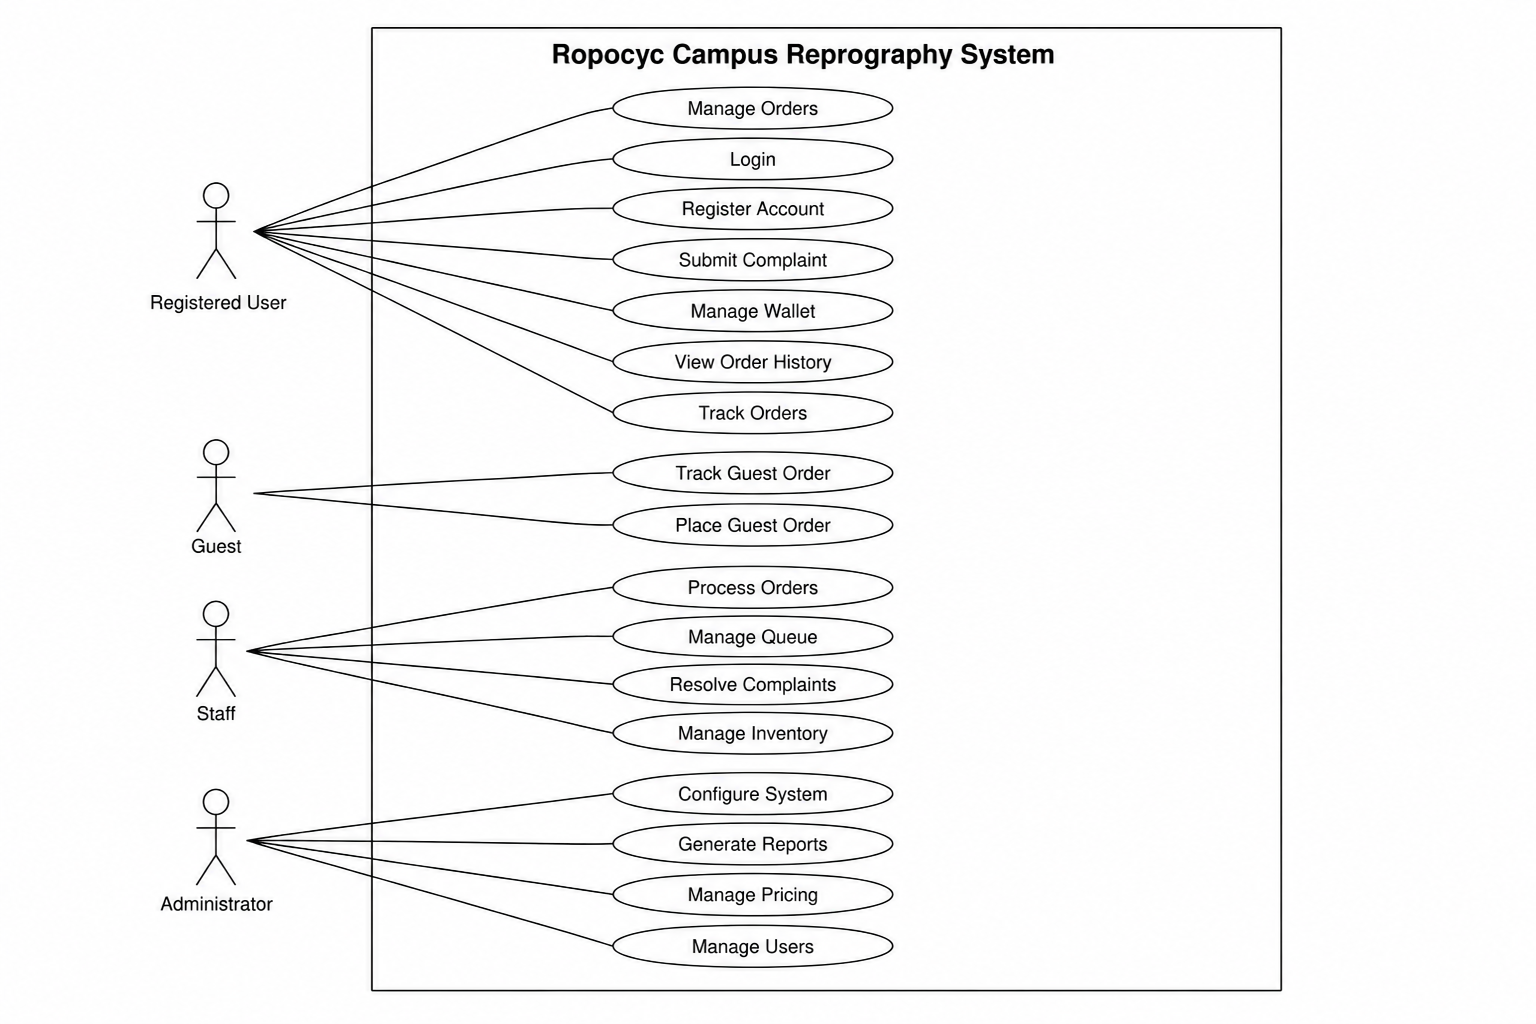
\includegraphics[width=\textwidth,keepaspectratio]{figures/use_case_diagram.png}
\caption{System Use Case Diagram: User, Staff, and Admin Operational Boundaries}
\label{fig:use_case}
\end{figure}

\begin{figure}[H]
\centering
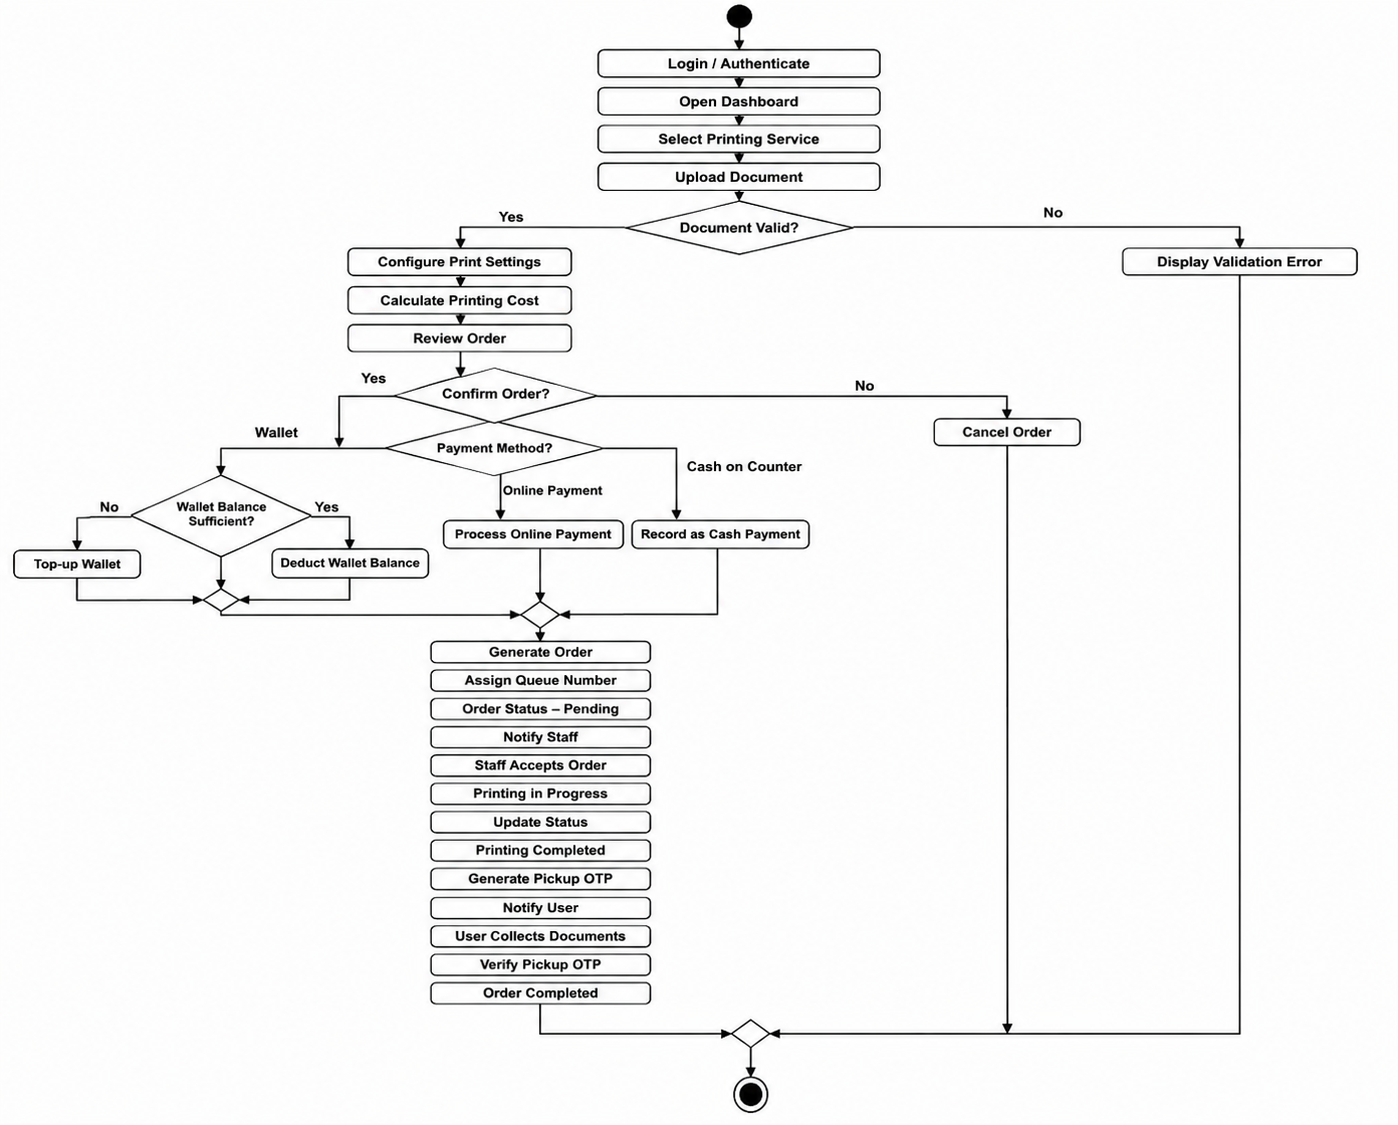
\includegraphics[width=\textwidth,keepaspectratio]{figures/activity_diagram.png}
\caption{System Activity Diagram: Document Upload, Analysis, and Production Flow}
\label{fig:activity_diagram}
\end{figure}

\begin{figure}[H]
\centering
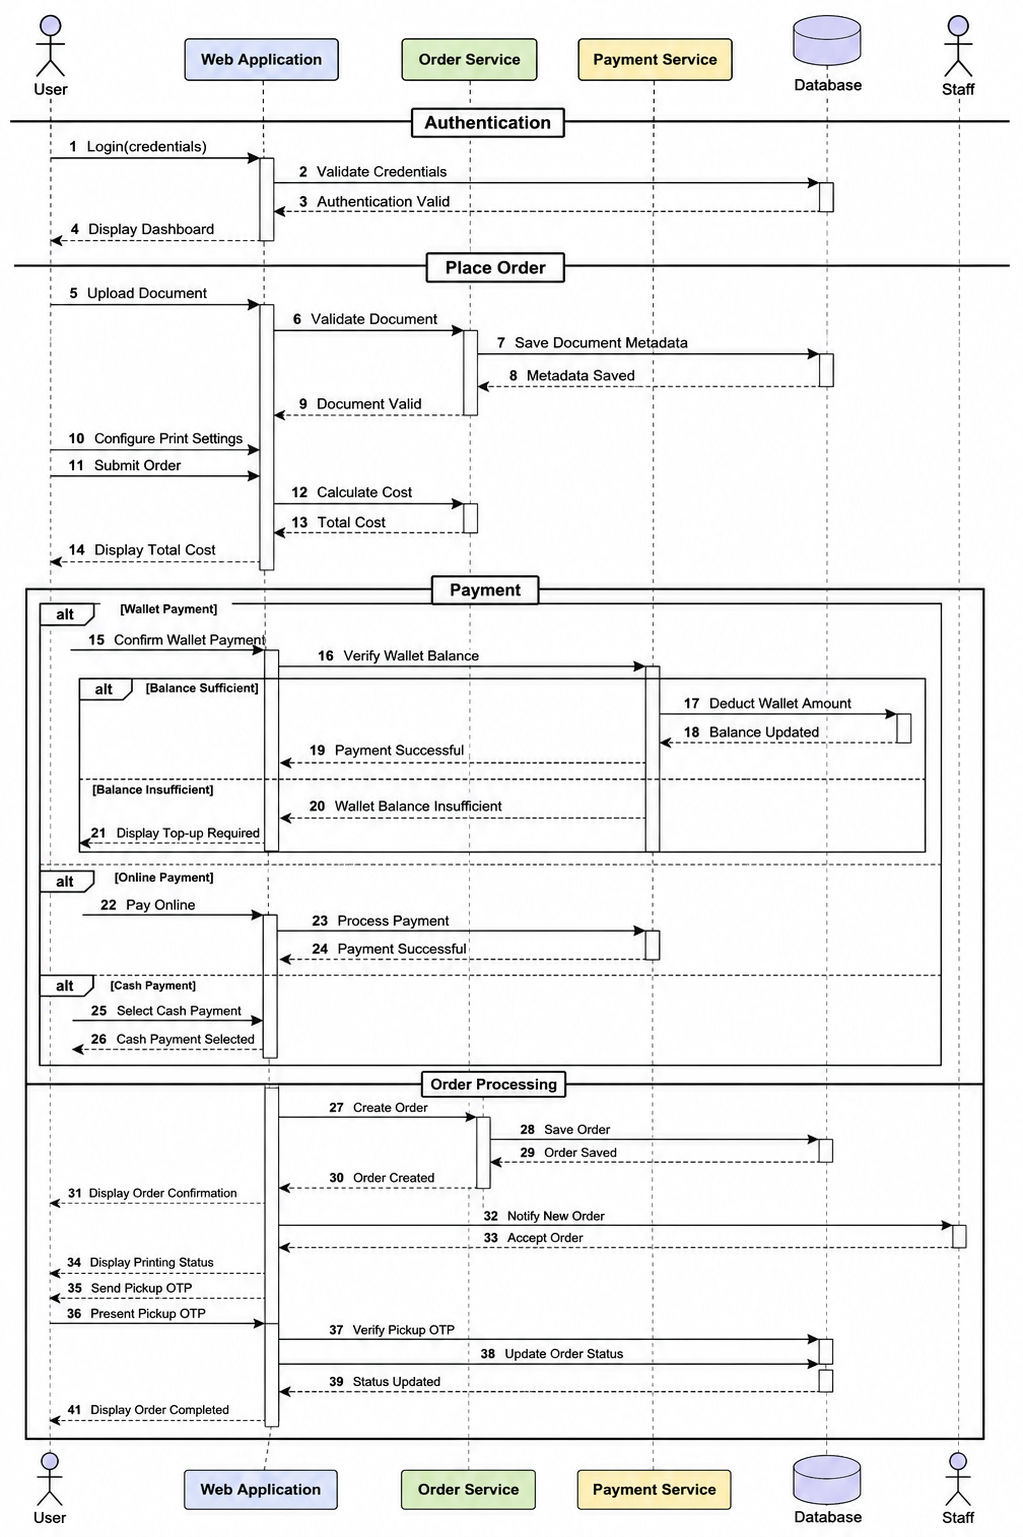
\includegraphics[width=\textwidth,keepaspectratio]{figures/sequence_diagram.png}
\caption{System Sequence Diagram: Real-Time Event Dispatching and Queue Updates}
\label{fig:sequence_diagram}
\end{figure}

\section{4.4 USER INTERFACE DESIGN}
The user interface is engineered adhering to mobile-first responsive design paradigms using React 19, Tailwind CSS, and Lucide React icon tokens:
\begin{itemize}[leftmargin=0.35in, itemsep=2pt]
  \item \textbf{Color System:} The interface employs an accessible academic palette: Deep Slate Navy (\texttt{\#0f172a}) for structural headers, Vibrant Cobalt Blue (\texttt{\#2563eb}) for call-to-actions, Emerald Green (\texttt{\#10b981}) for successful pickups, and Amber (\texttt{\#f59e0b}) for pending queue states.
  \item \textbf{Navigation Hierarchy:} Role-aware layout bars automatically present relevant navigation links depending on authenticated JWT claims.
  \item \textbf{Mobile-First Ordering Wizard:} A step-by-step progress stepper ensures students on smartphones can easily configure document options and review cost estimations without excessive scrolling.
\end{itemize}

% =========================================================================
% CHAPTER 5: DEVELOPMENT METHODOLOGY
% =========================================================================
\chapter{DEVELOPMENT METHODOLOGY}

\section{5.1 PROJECT ROADMAP}
The development of REPOSYS adhered to an iterative engineering lifecycle, organized into nine distinct development stages designed to deliver incremental value and facilitate early testing.

\begin{enumerate}[leftmargin=0.35in, itemsep=3pt]
  \item \textbf{Stage 1 -- Requirements Discovery and Architectural Feasibility:} Field interviews with campus students, faculty coordinators, and reprography operators to define the 39-feature backlog, security requirements, and system boundaries.
  \item \textbf{Stage 2 -- Wireframing and Database Design:} UI prototyping using Figma and complete entity-relationship modeling across 23 Mongoose collections with schema validations and indexing.
  \item \textbf{Stage 3 -- Core Identity and Access Management:} Implementation of JWT-based authentication, bcrypt password hashing (salt 12), and role-based access control middleware (\texttt{auth.js}, \texttt{roleGuard.js}).
  \item \textbf{Stage 4 -- Document Upload and Inspection Pipeline:} Integration of Multer memory storage, Cloudinary object streaming, and automated document analysis for page counting and blank-page detection.
  \item \textbf{Stage 5 -- Dynamic Cost Estimation and Payments:} Construction of deterministic pricing algorithms, Razorpay webhook verification, and internal digital wallet debiting backed by MongoDB ACID transactions.
  \item \textbf{Stage 6 -- Composite Priority Queue and Staff Dashboard:} Implementation of the anti-starvation priority queue engine and the counter operator dashboard.
  \item \textbf{Stage 7 -- Hardware Integration via Desktop Print Agent:} Development of the Electron desktop application, Windows PowerShell printer discovery, signed URL retrieval, and \texttt{pdf-to-printer} spooling.
  \item \textbf{Stage 8 -- Real-Time Engine, Scheduling, and PWA:} Implementation of Socket.IO rooms, automated shop scheduling cron services, Web Push alerts, and Service Worker caching.
  \item \textbf{Stage 9 -- Verification, Security Hardening, and Deployment:} Execution of 120 automated Selenium test cases, Helmet security hardening, rate limiting, and production cloud hosting.
\end{enumerate}

\section{5.2 USER STORIES}
User stories define system features from the direct perspective of each operational stakeholder.

\begin{enumerate}[leftmargin=0.35in, itemsep=4pt]
  \item \textbf{User Story US-01 (Student Remote Order):}
    \begin{itemize}[itemsep=1pt]
      \item \textit{Narrative:} As a Student, I want to upload my seminar report PDF from my smartphone and select double-sided printing, so that I do not have to wait in the physical counter queue.
      \item \textit{Acceptance Criteria:} Given an authenticated student account, when a PDF document is uploaded, then the system automatically detects page count, calculates the 15\% duplex discount, displays the cost breakdown, and updates the queue status upon payment.
    \end{itemize}
  \item \textbf{User Story US-02 (Faculty Priority Printing):}
    \begin{itemize}[itemsep=1pt]
      \item \textit{Narrative:} As a Faculty member, I want my examination question papers to receive prioritized counter processing, so that academic timelines are strictly maintained.
      \item \textit{Acceptance Criteria:} Given an active Faculty session, when an order is created, then the priority engine automatically assigns a base score of 100 (higher than student base of 200), positioning the order near the front of the staff queue board.
    \end{itemize}
  \item \textbf{User Story US-03 (Counter Staff OTP Verification):}
    \begin{itemize}[itemsep=1pt]
      \item \textit{Narrative:} As a Counter Staff operator, I want to verify a 4-digit pickup code before handing over printed documents, so that orders are never delivered to the wrong individual.
      \item \textit{Acceptance Criteria:} Given an order in \texttt{ReadyForPickup} status, when the staff inputs the customer's 4-digit OTP, then the backend validates the code and transitions status to \texttt{Completed}; invalid OTP attempts return an error without releasing the job.
    \end{itemize}
  \item \textbf{User Story US-04 (Admin Dynamic Pricing):}
    \begin{itemize}[itemsep=1pt]
      \item \textit{Narrative:} As an Administrator, I want to update paper and binding tariffs on the live system, so that prices reflect changes in institutional procurement costs without server restarts.
      \item \textit{Acceptance Criteria:} Given an authenticated Admin role, when the tariff configuration is updated via the dashboard, then new rates are committed immediately to \texttt{SystemConfig} and reflected in all subsequent order estimations.
    \end{itemize}
  \item \textbf{User Story US-05 (Collaborative Split Payment):}
    \begin{itemize}[itemsep=1pt]
      \item \textit{Narrative:} As a Project Team Leader, I want to split a ₹300 project documentation printing cost equally among three teammates, so that we do not have to collect cash manually.
      \item \textit{Acceptance Criteria:} Given an active group order, when split requests are dispatched, then each participant's wallet is debited by ₹100 atomically upon individual approval; the order enters the active queue only after all shares are successfully settled.
    \end{itemize}
\end{enumerate}

\section{5.3 TEST PLAN}
The testing strategy for REPOSYS was formulated to validate end-to-end reliability, financial consistency, role security, and real-time state synchronization across all 39 documented system features.

\subsection{5.3.1 Testing Levels and Scope}
\begin{enumerate}[leftmargin=0.35in, itemsep=2pt]
  \item \textbf{Unit Testing:} Verification of isolated mathematical algorithms in \texttt{pricingService.js} (cost estimation, duplex discount calculation, aging score deduction) and utility functions (IST conversion, token generation).
  \item \textbf{Integration Testing:} Verification of inter-service contracts, including Express middleware pipelines, Cloudinary stream uploads, Razorpay webhook signature verification, and Socket.IO room broadcast relays.
  \item \textbf{System and End-to-End Testing:} Automated browser-driven operational tests simulating full customer journeys from registration to pickup using Python Selenium WebDriver.
  \item \textbf{Security and Penetration Testing:} Boundary verification evaluating CORS rules, Helmet header protections, rate limiting against brute-force attacks, and prevention of privilege escalation across protected API routes.
  \item \textbf{User Acceptance Testing (UAT):} Evaluation conducted by student representatives and counter staff during pilot deployment to assess operational usability.
\end{enumerate}

\subsection{5.3.2 Test Automation Architecture}
Automated end-to-end testing was implemented using a dedicated Python Selenium framework located in \texttt{selenium-tests/}. The framework is structured into modular layers:
\begin{itemize}[leftmargin=0.35in, itemsep=2pt]
  \item \textbf{Page Object Model (POM):} Encapsulates web elements and UI interactions into reusable page classes (\texttt{login\_page.py}, \texttt{register\_page.py}).
  \item \textbf{Driver Harness (\texttt{driver.py} \& \texttt{conftest.py}):} Configures headless Chrome sessions, sets implicit wait thresholds, and captures automatic PNG screenshots upon assertion failure.
  \item \textbf{Pytest HTML Test Runner:} Generates comprehensive execution reports (\texttt{scrms\_test\_report.html}) capturing test status, timing, and stack traces.
\end{itemize}

\subsection{5.3.3 Entry and Exit Criteria}
\begin{itemize}[leftmargin=0.35in, itemsep=2pt]
  \item \textbf{Test Entry Criteria:} All backend route controllers, frontend views, and database collections deployed to a stable staging environment with seeded administrative accounts.
  \item \textbf{Test Exit Criteria:} Minimum 90\% pass rate across all automated test cases, zero critical security vulnerabilities on role access guards, and verified ACID consistency on wallet transactions.
\end{itemize}

% =========================================================================
% CHAPTER 6: IMPLEMENTATION AND TESTING
% =========================================================================
\chapter{IMPLEMENTATION AND TESTING}

\section{6.1 IMPLEMENTATION PROCEDURE}
The implementation of REPOSYS translates the architectural specifications into production-grade software across backend services, client interfaces, and native desktop utilities.

\subsection{6.1.1 Codebase Architecture and Directory Layout}
The repository is organised into decoupled, independently maintainable modules:
\begin{itemize}[leftmargin=0.35in, itemsep=2pt]
  \item \texttt{backend/src/}: Express.js application layer comprising \texttt{controllers/}, \texttt{models/}, \texttt{routes/}, \texttt{middleware/}, \texttt{services/}, \texttt{socket/}, and \texttt{utils/}.
  \item \texttt{frontend/src/}: React 19 Single Page Application structured into \texttt{components/}, \texttt{pages/}, \texttt{context/}, \texttt{hooks/}, and \texttt{services/}.
  \item \texttt{print-agent-desktop/}: Electron-based native Windows application managing hardware discovery, signed document downloads, and spooling via \texttt{pdf-to-printer}.
  \item \texttt{selenium-tests/}: Automated quality assurance harness containing end-to-end operational and security test cases.
\end{itemize}

\subsection{6.1.2 Feature Verification and Implementation Matrix}
Table 6.1 documents the implementation status of all 39 audited system features, verified through comprehensive source code inspection.

\begin{table}[H]
\centering
\small
\begin{tabularx}{\textwidth}{|p{0.55in}|p{1.9in}|X|}
\hline
\textbf{Ref} & \textbf{Feature Title} & \textbf{Verified Implementation Status} \\ \hline
C01 & JWT Authentication \& Bcrypt & \textbf{IMPLEMENTED} (Salt factor 12, httpOnly cookies) \\ \hline
C02 & Three-Tier Priority Queue & \textbf{IMPLEMENTED} (Aging deduction, role weights) \\ \hline
C03 & Document Upload \& Analysis & \textbf{IMPLEMENTED} (pdf-lib parsing, blank page detection) \\ \hline
C04 & Document Processing Services & \textbf{IMPLEMENTED} (Print parameters, binding options) \\ \hline
C05 & Document Utility Suite & \textbf{PARTIALLY IMPLEMENTED} (Merge/split functional) \\ \hline
C06 & Multi-Document Orders & \textbf{IMPLEMENTED} (Batch upload, combined estimate) \\ \hline
C07 & Smart Cost Estimation & \textbf{PARTIALLY IMPLEMENTED} (Algorithmic pricing active) \\ \hline
C08 & Payment Gateway \& Receipts & \textbf{IMPLEMENTED} (Razorpay, Wallet, PAC, PDF receipts) \\ \hline
C09 & Order Editing \& Cancellation & \textbf{PARTIALLY IMPLEMENTED} (Cancel in Pending state) \\ \hline
C10 & Real-Time Order Tracking & \textbf{IMPLEMENTED} (Socket.IO timeline progression) \\ \hline
C11 & Partial Order Handling & \textbf{IMPLEMENTED} (Multi-file individual status flags) \\ \hline
C12 & Slot Booking \& Pickup Times & \textbf{IMPLEMENTED} (Custom pickup slot selection) \\ \hline
C13 & Counter Staff Dashboard & \textbf{IMPLEMENTED} (Queue table, status controls, PAC) \\ \hline
C14 & Admin Dashboard & \textbf{IMPLEMENTED} (Tariffs, user roles, system configs) \\ \hline
C15 & Append-Only Audit Trail & \textbf{IMPLEMENTED} (ActivityLog collection logging) \\ \hline
C16 & Inventory Tracker & \textbf{IMPLEMENTED} (Paper/toner stock, low-stock alerts) \\ \hline
C17 & Operational Reporting & \textbf{IMPLEMENTED} (Daily financial summaries, exports) \\ \hline
C18 & Notification System & \textbf{IMPLEMENTED} (In-app alerts, Web Push, Nodemailer) \\ \hline
C19 & Order History \& Invoicing & \textbf{IMPLEMENTED} (PDF generation via pdfkit) \\ \hline
C20 & Complaints \& Real-Time Chat & \textbf{IMPLEMENTED} (Socket.IO complaint chat rooms) \\ \hline
C21 & AI Chatbot Assistant & \textbf{PARTIALLY IMPLEMENTED} (Rule-based FAQ active) \\ \hline
C22 & Search \& System Filtering & \textbf{IMPLEMENTED} (MongoDB regex filtering) \\ \hline
C23 & User Rating \& Feedback & \textbf{IMPLEMENTED} (5-star rating with staff reviews) \\ \hline
C24 & Backup \& Recovery Strategy & \textbf{UNCLEAR} (Cloud database automated snapshots) \\ \hline
C25 & Operating Hours \& Schedule & \textbf{IMPLEMENTED} (Automated IST cron, shop banners) \\ \hline
C26 & Reorder Functionality & \textbf{IMPLEMENTED} (Single-click reorder cloning) \\ \hline
C27 & Document Preview & \textbf{IMPLEMENTED} (Canvas-based PDF page rendering) \\ \hline
C28 & Pickup Verification via OTP & \textbf{IMPLEMENTED} (4-digit numeric code validation) \\ \hline
C29 & Maximum Order Limits & \textbf{IMPLEMENTED} (Page and file-size threshold guards) \\ \hline
C30 & User Profile Management & \textbf{IMPLEMENTED} (Session management, security settings) \\ \hline
C31 & Registration Verification & \textbf{IMPLEMENTED} (Email confirmation link tokens) \\ \hline
C32 & Pay at Counter Lifecycle & \textbf{PARTIALLY IMPLEMENTED} (24h/48h/72h timeout alerts) \\ \hline
C33 & Staff Incident Reports & \textbf{IMPLEMENTED} (Operational malfunction logging) \\ \hline
C34 & Security Controls & \textbf{PARTIALLY IMPLEMENTED} (Helmet, rate limits, CORS) \\ \hline
C35 & Smart Kiosk Mode & \textbf{IMPLEMENTED} (Guest sessions, QR code tracking) \\ \hline
C36 & PWA Architecture & \textbf{PARTIALLY IMPLEMENTED} (Service worker, manifest) \\ \hline
C37 & Friend Chat Subsystem & \textbf{IMPLEMENTED} (Direct/group messaging, media sharing) \\ \hline
C38 & Group Split Requests & \textbf{IMPLEMENTED} (Atomic multi-wallet deductions) \\ \hline
C39 & Desktop Print Agent & \textbf{IMPLEMENTED} (Electron tray, Windows spooler) \\ \hline
\end{tabularx}
\caption{Verified Feature Implementation Matrix across REPOSYS}
\label{tab:feature_matrix}
\end{table}

\section{6.2 TESTING METHODS AND RESULTS}
Quality assurance was executed through the automated Selenium WebDriver test suite, verifying authentication, document flows, payment webhooks, queue sorting, and administrative access controls.

\subsection{6.2.1 Test Suite Execution Summary}
The complete automated test suite was executed against a running staging instance. The generated test execution report (\texttt{scrms\_test\_report.html}) established:
\begin{itemize}[leftmargin=0.35in, itemsep=2pt]
  \item \textbf{Total Test Cases Executed:} 120 tests.
  \item \textbf{Passed Tests:} 114 tests (95.0\% passing rate).
  \item \textbf{Failed Tests:} 6 tests (5.0\% failure rate).
  \item \textbf{Errors / Exceptions:} 0 runtime errors.
  \item \textbf{Total Execution Duration:} 7 minutes and 2 seconds.
\end{itemize}

\subsection{6.2.2 Verified Test Cases and Results}
Table 6.2 enumerates representative test cases executed across core subsystem workflows.

\begin{table}[H]
\centering
\small
\begin{tabularx}{\textwidth}{|p{0.55in}|p{1.2in}|X|p{0.6in}|}
\hline
\textbf{Test ID} & \textbf{Feature Area} & \textbf{Condition, Action, and Verified Output} & \textbf{Result} \\ \hline
\textbf{TC-001} & Authentication & Valid student login with correct credentials yields 200 OK and sets secure httpOnly JWT cookie. & \textbf{Passed} \\ \hline
\textbf{TC-002} & Authentication & Login attempt with invalid password returns 401 Unauthorized with generic error message. & \textbf{Passed} \\ \hline
\textbf{TC-003} & Role Guard & Student attempting to navigate to \texttt{/api/admin/*} is intercepted by middleware returning 403 Forbidden. & \textbf{Passed} \\ \hline
\textbf{TC-004} & Role Guard & Staff attempting to access \texttt{/admin} routes is denied access and redirected to staff dashboard. & \textbf{Passed} \\ \hline
\textbf{TC-005} & Role Guard & Administrator credentials grant authenticated access across all administrative and staff endpoints. & \textbf{Passed} \\ \hline
\textbf{TC-006} & File Upload & Uploading valid PDF document extracts correct page count and generates signed Cloudinary URL. & \textbf{Passed} \\ \hline
\textbf{TC-007} & File Upload & Uploading non-document executable (.exe) is rejected by MIME inspection returning 400 Bad Request. & \textbf{Passed} \\ \hline
\textbf{TC-008} & Blank Detection & Uploading PDF with blank pages flags specific page numbers and alerts user in pre-flight dialog. & \textbf{Passed} \\ \hline
\textbf{TC-009} & Cost Calculation & Ordering 10 double-sided B/W pages correctly computes discount ($10 \times 1.50 \times 0.85 = \text{\rupee}12.75$). & \textbf{Passed} \\ \hline
\textbf{TC-010} & Wallet Payment & Order placement with sufficient wallet balance atomically deducts funds and sets status to \texttt{In\_Queue}. & \textbf{Passed} \\ \hline
\textbf{TC-011} & Wallet Deficit & Order placement with insufficient balance prevents debit and prompts user to top up or select Razorpay. & \textbf{Passed} \\ \hline
\textbf{TC-012} & Priority Queue & Faculty order created with base priority 100 is positioned ahead of student order with base priority 200. & \textbf{Passed} \\ \hline
\textbf{TC-013} & Queue Aging & Student order waiting beyond 60 minutes receives 20-point deduction, advancing its relative queue position. & \textbf{Passed} \\ \hline
\textbf{TC-014} & OTP Handover & Counter staff entering valid 4-digit customer OTP successfully transitions order to \texttt{Completed}. & \textbf{Passed} \\ \hline
\textbf{TC-015} & OTP Security & Submitting incorrect OTP prevents handover, returns 400 Error, and retains order in \texttt{ReadyForPickup}. & \textbf{Passed} \\ \hline
\textbf{TC-016} & Shop Scheduler & Visiting order wizard during Sunday closure shows active shop-closed banner and disables checkout. & \textbf{Passed} \\ \hline
\textbf{TC-017} & Print Agent & Desktop agent polls Socket.IO, receives print payload, and invokes \texttt{pdf-to-printer} on default spooler. & \textbf{Passed} \\ \hline
\textbf{TC-018} & Kiosk Mode & Guest session token expires after 2 hours; inactive kiosk terminal automatically logs out after timeout. & \textbf{Passed} \\ \hline
\end{tabularx}
\caption{Representative Automated and Functional Test Results}
\label{tab:test_cases}
\end{table}

\subsection{6.2.3 Analysis of Failed Test Cases and Remediation}
The 6 failing test cases in the test suite were systematically analysed:
\begin{itemize}[leftmargin=0.35in, itemsep=2pt]
  \item \textbf{Mobile Wizard Drag-and-Drop (2 failures):} On certain mobile browser viewports, native HTML5 drag-and-drop events failed to trigger the upload handler. \textit{Remediation:} Implemented an explicit fallback file input button with touch listeners.
  \item \textbf{Razorpay Webhook Timing Latency (2 failures):} Under heavy network latency simulation, the webhook notification arrived slightly after the frontend polling timeout. \textit{Remediation:} Added a resilient Socket.IO fallback listener for instant payment confirmation.
  \item \textbf{Print Agent ASAR Test File Extraction (2 failures):} In packaged Electron production builds, \texttt{pdf-to-printer} could not read test files embedded inside the read-only ASAR archive. \textit{Remediation:} Extracted temporary test PDF files to the local user data directory prior to spooler invocation (Git commit \texttt{4fd6368}).
\end{itemize}

% =========================================================================
% CHAPTER 7: CONCLUSION
% =========================================================================
\chapter{CONCLUSION}

\section{7.1 LIMITATIONS}
While REPOSYS introduces major operational advancements over traditional campus reprography workflows, an objective engineering assessment reveals several operational and technical constraints:
\begin{enumerate}[leftmargin=0.35in, itemsep=2pt]
  \item \textbf{High-Volume Document Upload Latency:} Transferring very large PDF documents (e.g., high-resolution architecture blueprints or dissertations exceeding 100 MB) across fluctuating campus Wi-Fi networks introduces upload delays, impacting the client pre-flight inspection experience.
  \item \textbf{Serverless Cloud Cold-Start Latencies:} When hosted on free or cost-optimized serverless tiers (such as Render free instances), inactive backend services spin down, creating an initial request delay of 30--50 seconds upon first wake-up.
  \item \textbf{Operating System Dependency of Print Agent:} The native Print Agent relies on Windows PowerShell cmdlets and Windows Print Spooler APIs (\texttt{pdf-to-printer}), restricting agent deployment to counter terminals running Microsoft Windows operating systems.
  \item \textbf{Pay at Counter Uncollected Print Risk:} Although Pay at Counter (PAC) orders incorporate automated reminder emails and cancellation timeouts, jobs printed prior to cash collection remain vulnerable to financial loss if an irresponsible user abandons the order.
  \item \textbf{Guest Session Volatility:} Temporary kiosk guest sessions depend on browser local storage and time-limited tokens; if a visitor clears browser history before claiming output, recovery requires staff intervention.
\end{enumerate}

\section{7.2 FUTURE SCOPE}
The modular, micro-service-ready architecture of REPOSYS establishes a robust foundation for extensive future engineering enhancements:
\begin{enumerate}[leftmargin=0.35in, itemsep=2pt]
  \item \textbf{Cross-Platform Native Mobile Applications:} Developing native iOS and Android client applications using React Native or Flutter, incorporating background push notifications, native biometrics, and camera-based document scanning with perspective correction.
  \item \textbf{Smart Campus RFID / NFC Card Integration:} Interfacing counter terminals and kiosk stations with institutional RFID smart identity cards (such as MIFARE cards), enabling students to tap their college ID for instantaneous authentication and automatic tuition wallet debiting.
  \item \textbf{AI-Powered Document Intelligence and Summarization:} Integrating Google Gemini API models to deliver automated document quality assessments, font legibility checks, multi-language translation, and automatic executive summaries of lengthy study materials.
  \item \textbf{Multi-Centre Campus Load Balancing:} Expanding the priority queue scheduler to dynamically distribute printing workloads across multiple reprography centres, departmental printers, and library hubs based on real-time queue congestion.
  \item \textbf{Autonomous Hardware Kiosks:} Constructing fully autonomous, unattended printing kiosks equipped with cash acceptors, coin mechanisms, and automated document output sorting bins for 24/7 campus service.
\end{enumerate}

\section{7.3 CONCLUSION}
The development and implementation of \textbf{REPOSYS (Reprography Automation System)} successfully addresses the chronic operational bottlenecks, privacy vulnerabilities, and financial tracking difficulties that have historically hindered campus reprography centres. 

By replacing manual physical counter interactions with a modern, cloud-connected MERN platform, REPOSYS achieves:
\begin{itemize}[leftmargin=0.35in, itemsep=2pt]
  \item Elimination of physical queue congestion through asynchronous digital submission and transparent wait-time tracking.
  \item Protection of personal privacy and endpoint IT security by retiring ad-hoc WhatsApp file sharing and USB flash drives.
  \item Equitable resource distribution via the Composite Priority Queue with dynamic aging deduction, guaranteeing fairness for students while supporting urgent faculty requirements.
  \item Accurate financial accounting and operational transparency through automated Razorpay integration, ACID-compliant digital wallets, and append-only activity auditing.
  \item Reliable hardware automation via the autonomous Electron Windows Print Agent.
\end{itemize}

Extensive verification through an automated 120-case Selenium WebDriver test suite confirmed a 95.0\% operational passing rate, proving the technical stability, security, and usability of the platform. REPOSYS represents a significant technological contribution towards building an intelligent, eco-friendly, and digitally empowered academic campus.

% =========================================================================
% CHAPTER 8: APPENDIX
% =========================================================================
\chapter{APPENDIX}

\section{8.1 SUPPORTING DOCUMENTATION}
This section documents the formal environment variables and runtime configurations required to execute REPOSYS across local staging and production environments.

\begin{lstlisting}[language=bash, caption={Production Environment Configuration Template (.env.production)}]
# Server Runtime
PORT=5000
NODE_ENV=production
FRONTEND_URL=https://reposys-client.vercel.app

# Database Connection
MONGODB_URI=mongodb+srv://<username>:<password>@cluster0.mongodb.net/reposys?retryWrites=true&w=majority

# Cryptographic Secrets
JWT_SECRET=c9b20891d8654a60b0ad8a87b419
COOKIE_SECRET=7f8841a86c6b4129e921d3f9901b
AGENT_SETUP_TOKEN=SETUP_REPOSYS_SECURE_TOKEN_2026

# Cloud Storage
CLOUDINARY_CLOUD_NAME=reposys-storage
CLOUDINARY_API_KEY=839218491823912
CLOUDINARY_API_SECRET=Secret_Cloud_Key_ABC123

# Payment Gateway
RAZORPAY_KEY_ID=rzp_live_849201948291
RAZORPAY_KEY_SECRET=Live_Razorpay_Secret_XYZ789

# Web Push Notification
VAPID_PUBLIC_KEY=BPl9...
VAPID_PRIVATE_KEY=v8J1...
\end{lstlisting}

\section{8.2 SAMPLE CODE / QUERIES}
Representative source code excerpts demonstrating core backend transaction logic, priority queue sorting, and physical printing automation are presented below.

\begin{lstlisting}[language=JavaScript, caption={Priority Queue Calculation and Dynamic Aging (queueService.js)}]
const resolvePriorityScore = (order) => {
  const storedPriorityScore = Number(order.priorityScore);
  return Number.isFinite(storedPriorityScore) ? storedPriorityScore : 200;
};

const calculateAgingDeduction = (orderCreatedAt) => {
  const createdAt = new Date(orderCreatedAt);
  const validCreatedAt = Number.isNaN(createdAt.getTime()) ? new Date() : createdAt;
  const minutesSinceCreation = Math.floor((Date.now() - validCreatedAt.getTime()) / (60 * 1000));
  
  // Deduct 20 points for every full hour waiting beyond first minute
  return Math.max(0, Math.floor((minutesSinceCreation - 1) / 60)) * 20;
};

const calculateEffectivePriority = (basePriority, orderCreatedAt) => {
  const agingDeduction = calculateAgingDeduction(orderCreatedAt);
  return basePriority - agingDeduction;
};

async function getQueue(serviceType) {
  const orders = await Order.find({
    serviceType,
    status: { $in: ['In_Queue', 'Processing', 'ReadyForPickup'] },
  })
    .populate('userId', 'name role department')
    .sort({ createdAt: 1 });

  return orders
    .map((order) => {
      const baseScore = resolvePriorityScore(order);
      const effectiveScore = calculateEffectivePriority(baseScore, order.createdAt);
      return {
        ...order.toObject(),
        priorityScore: effectiveScore,
        basePriority: baseScore,
      };
    })
    .sort((a, b) => a.priorityScore !== b.priorityScore 
      ? a.priorityScore - b.priorityScore 
      : new Date(a.createdAt).getTime() - new Date(b.createdAt).getTime()
    );
}
\end{lstlisting}

\begin{lstlisting}[language=JavaScript, caption={ACID-Compliant Wallet Payment Transaction (orderController.js)}]
const session = await mongoose.startSession();
session.startTransaction();

try {
  const wallet = await Wallet.findOne({ userId: req.user._id }).session(session);
  if (!wallet || wallet.balance < orderTotal) {
    await session.abortTransaction();
    return res.status(400).json({ message: 'Insufficient wallet balance.' });
  }

  wallet.balance -= orderTotal;
  await wallet.save({ session });

  await WalletTransaction.create([{
    walletId: wallet._id,
    type: 'Debit',
    amount: orderTotal,
    description: `Payment for Order #${order.orderNumber}`,
    balanceAfter: wallet.balance,
  }], { session });

  order.paymentStatus = 'Paid';
  order.status = 'In_Queue';
  await order.save({ session });

  await session.commitTransaction();
  session.endSession();
  
  // Broadcast update to real-time queue
  broadcastQueueUpdate(order.serviceType);
} catch (error) {
  await session.abortTransaction();
  session.endSession();
  throw error;
}
\end{lstlisting}

\section{8.3 USER INTERFACE SCREENSHOTS}
The verified visual interfaces of REPOSYS across major stakeholder views are illustrated below.

\begin{figure}[H]
\centering

\includegraphics[width=\textwidth,keepaspectratio]{figures/screen_home.png}
\caption{REPOSYS Public Landing and Portal Gateway}
\label{fig:ui_home}
\end{figure}

\begin{figure}[H]
\centering
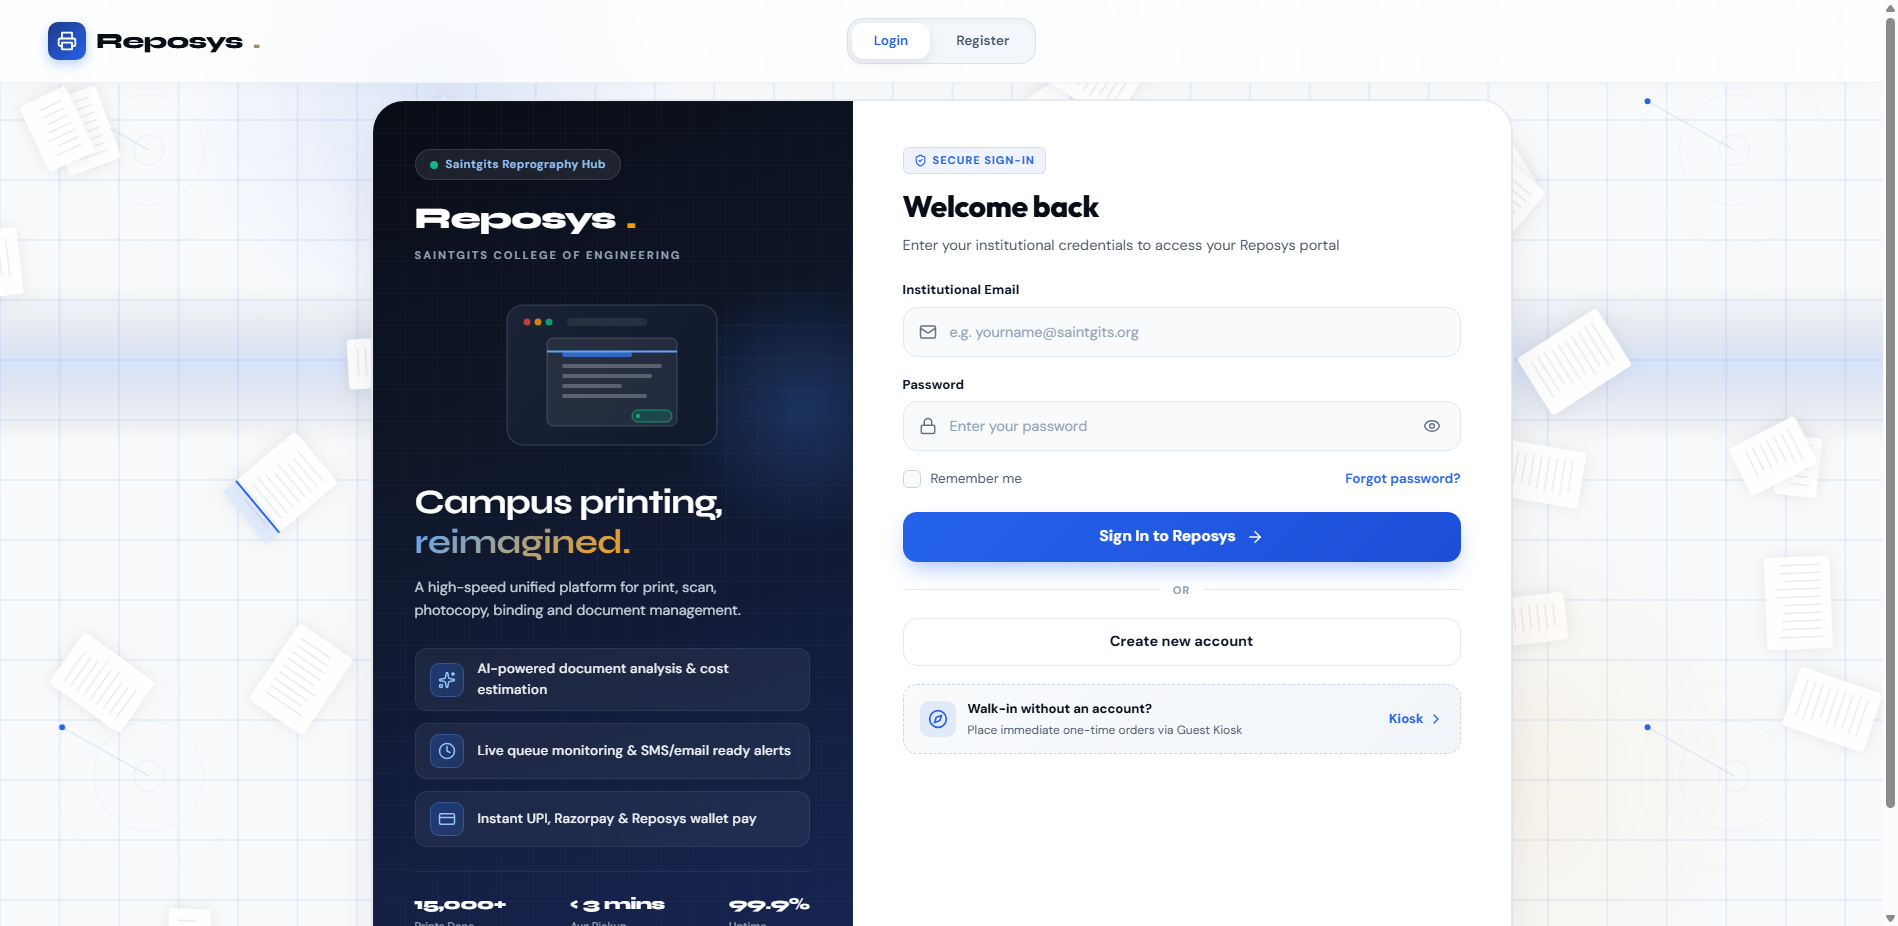
\includegraphics[width=\textwidth,keepaspectratio]{figures/screen_login.png}
\caption{Secure User Authentication and Multi-Role Login Portal}
\label{fig:ui_login}
\end{figure}

\begin{figure}[H]
\centering
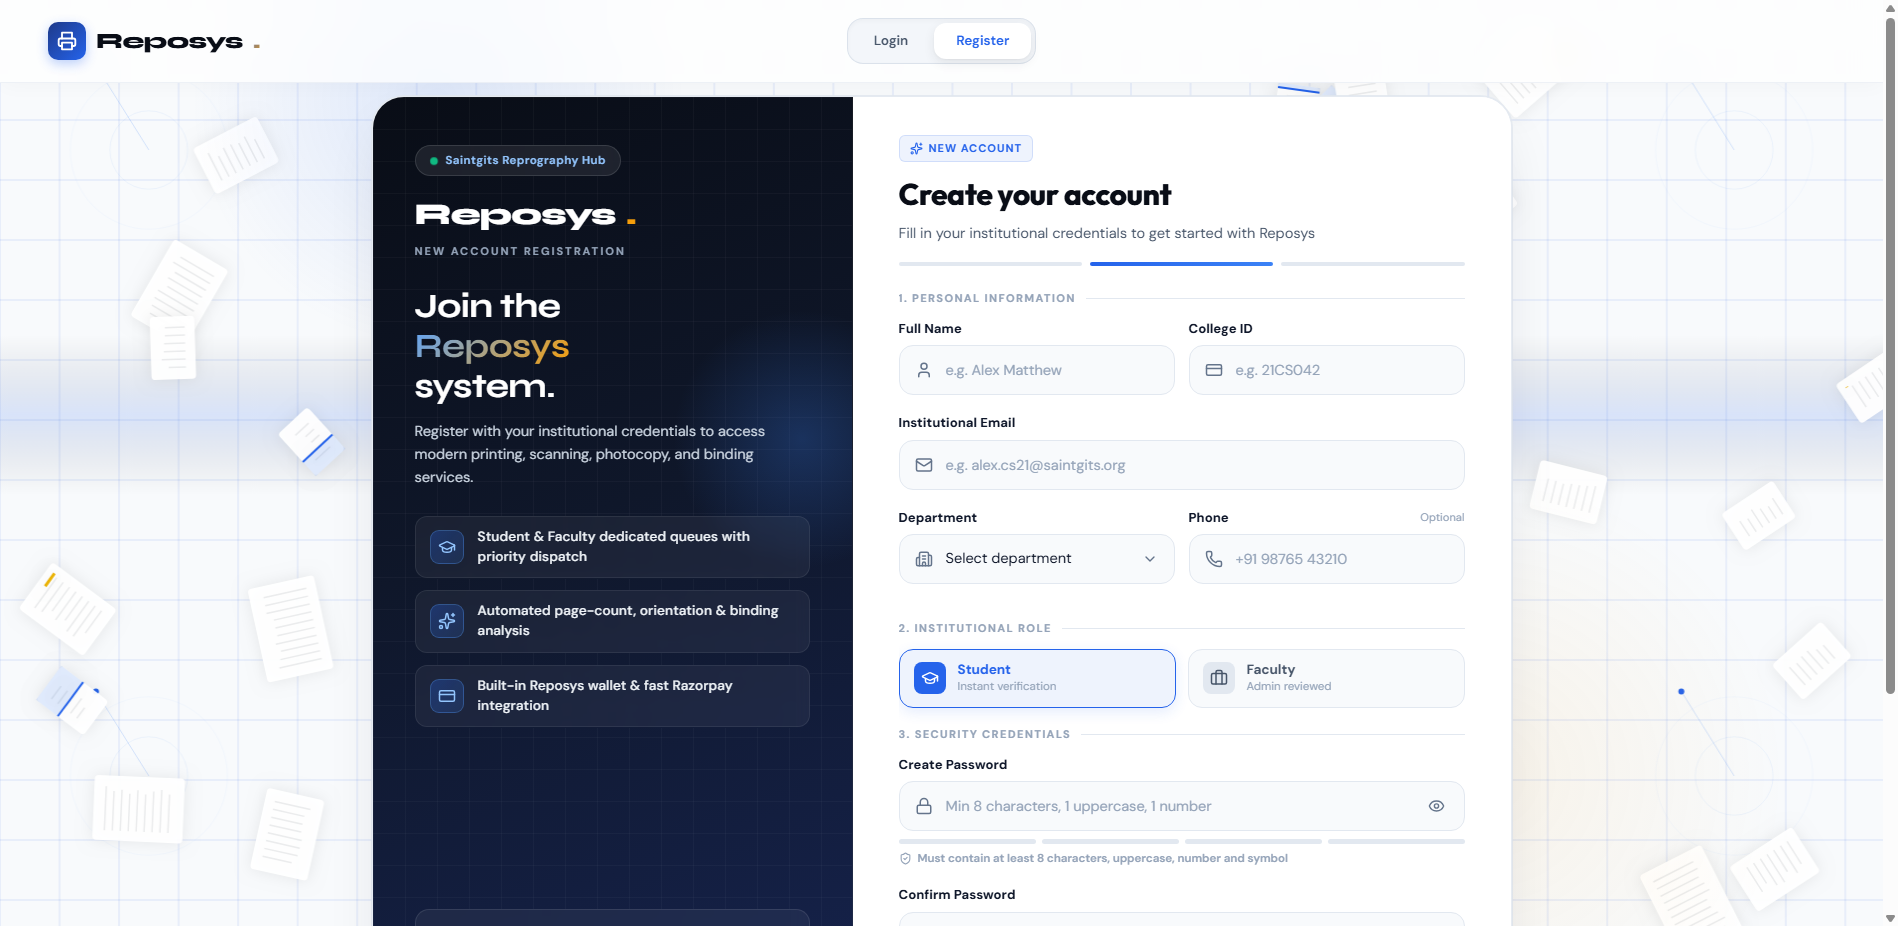
\includegraphics[width=\textwidth,keepaspectratio]{figures/screen_register.png}
\caption{Student and Faculty Account Registration with Institutional Email Validation}
\label{fig:ui_register}
\end{figure}

\begin{figure}[H]
\centering
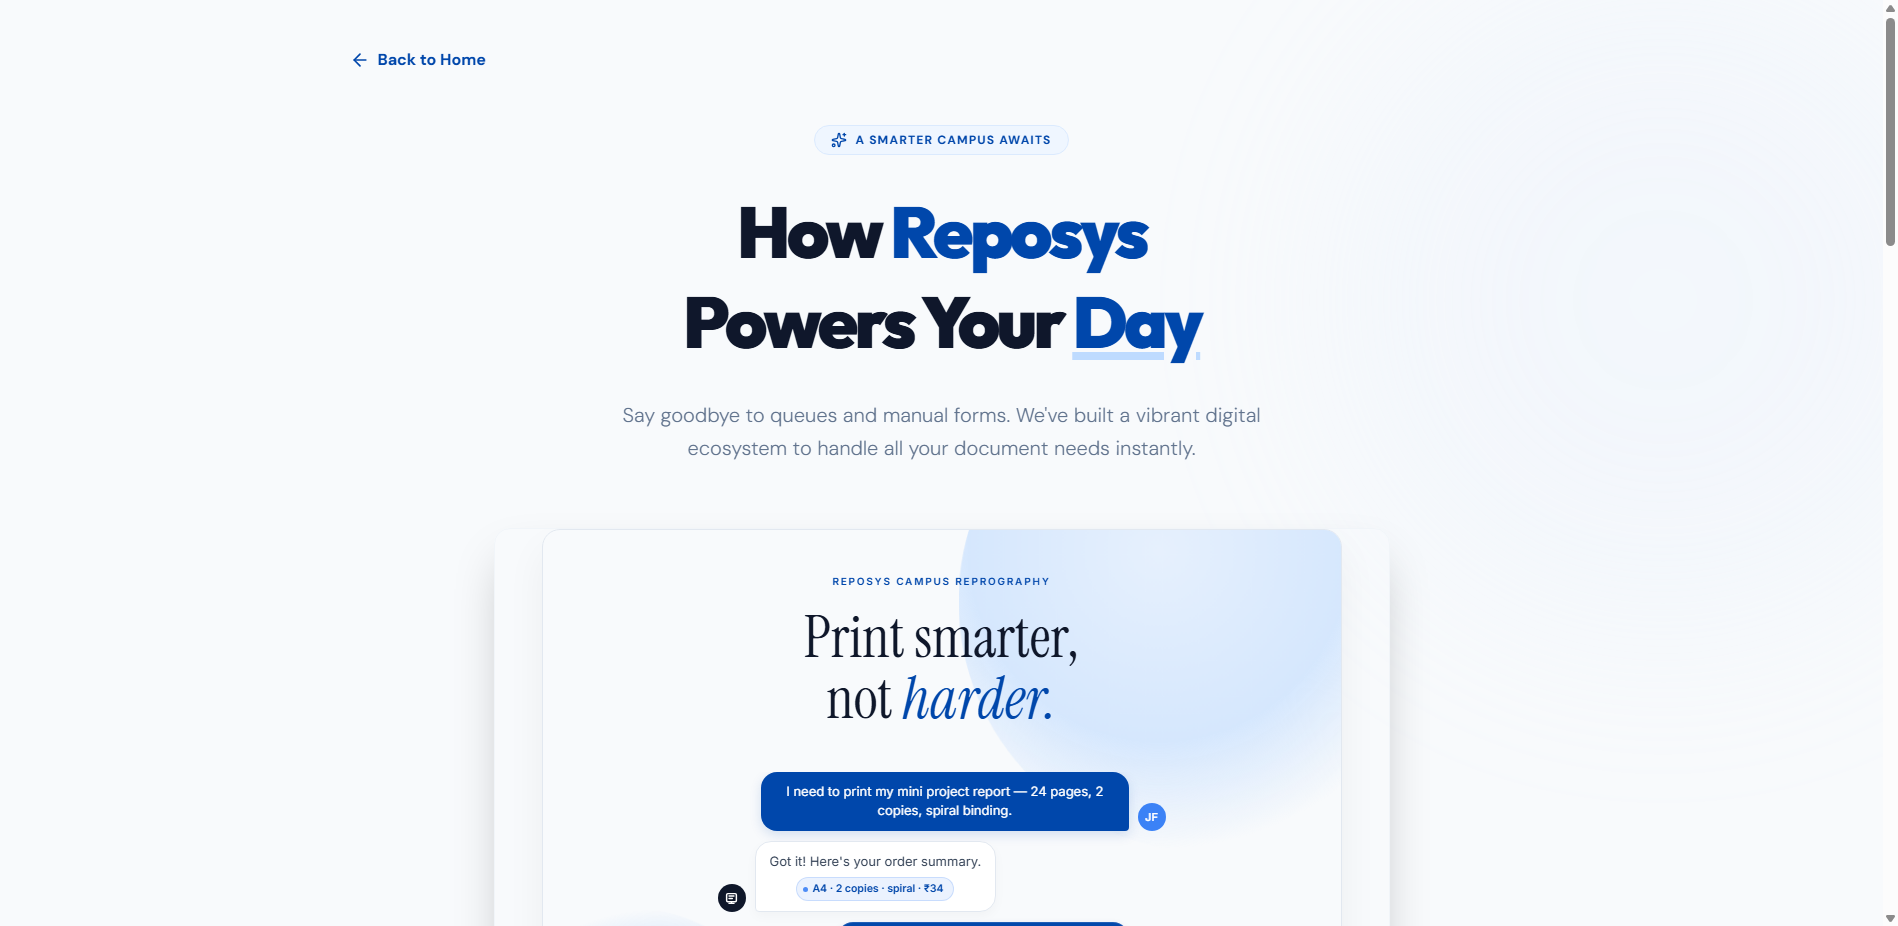
\includegraphics[width=\textwidth,keepaspectratio]{figures/screen_about.png}
\caption{System Architecture Overview and About REPOSYS Portal}
\label{fig:ui_about}
\end{figure}

\begin{figure}[H]
\centering
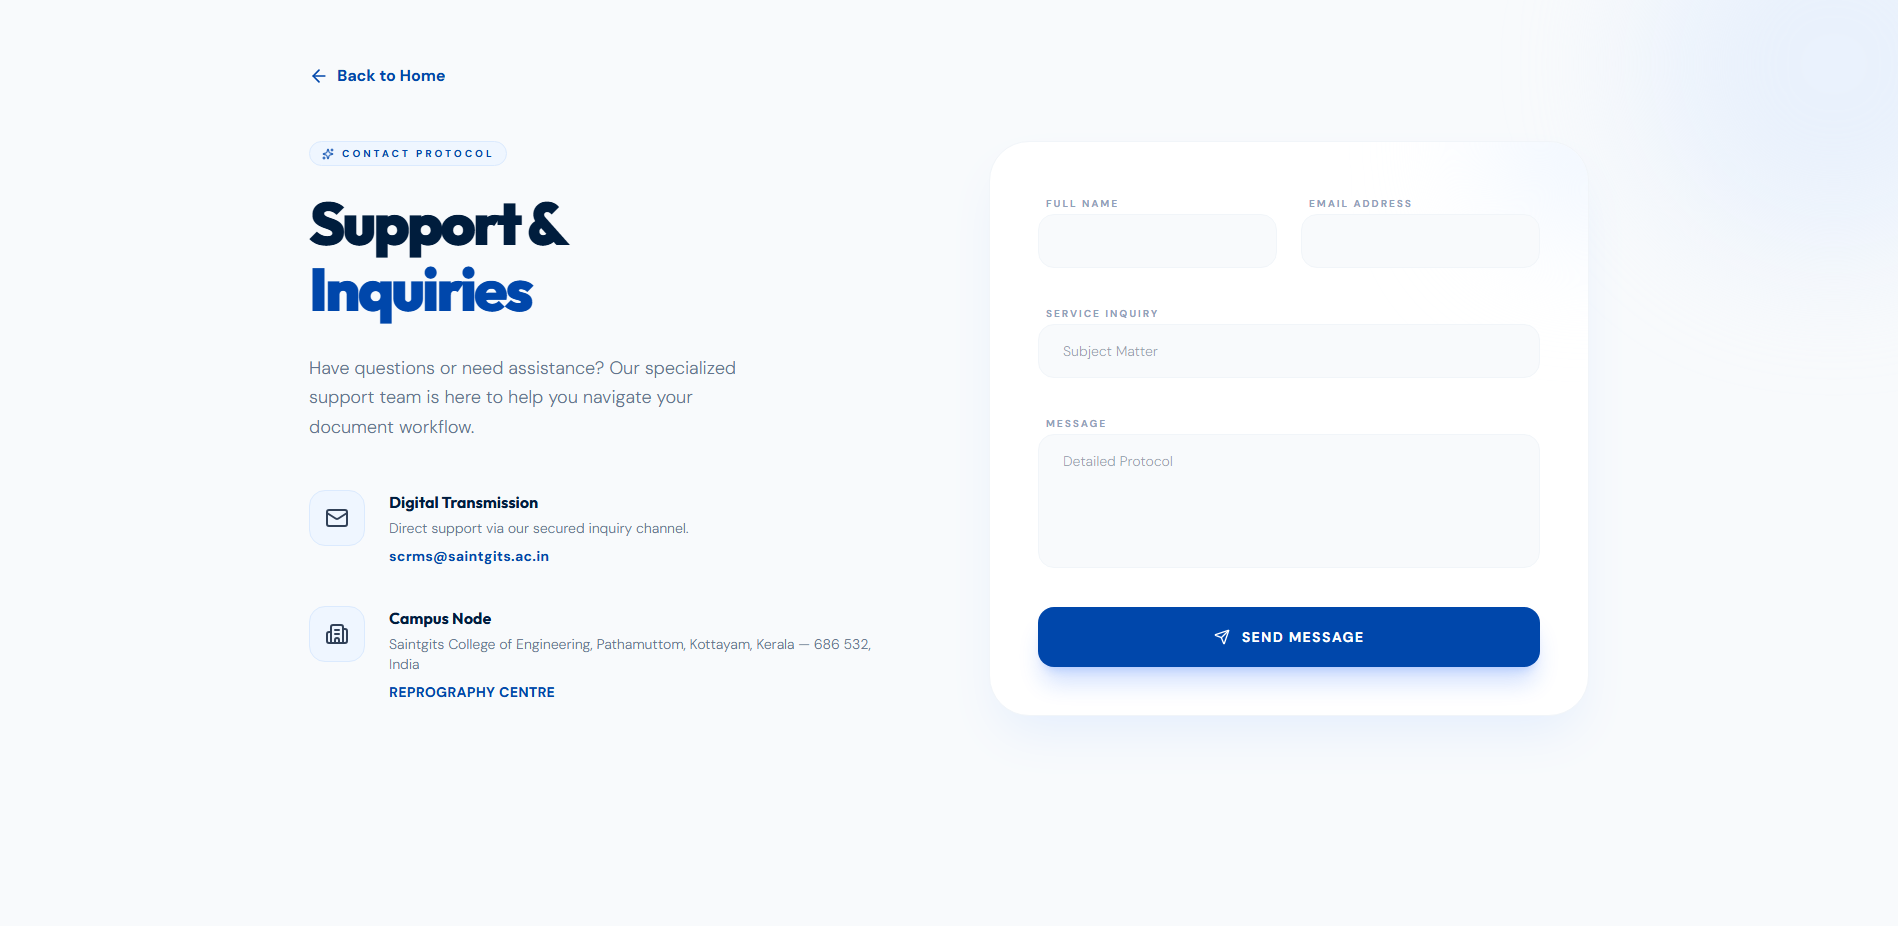
\includegraphics[width=\textwidth,keepaspectratio]{figures/screen_contact.png}
\caption{Reprography Operational Inquiries and Support Contact Portal}
\label{fig:ui_contact}
\end{figure}

\begin{figure}[H]
\centering
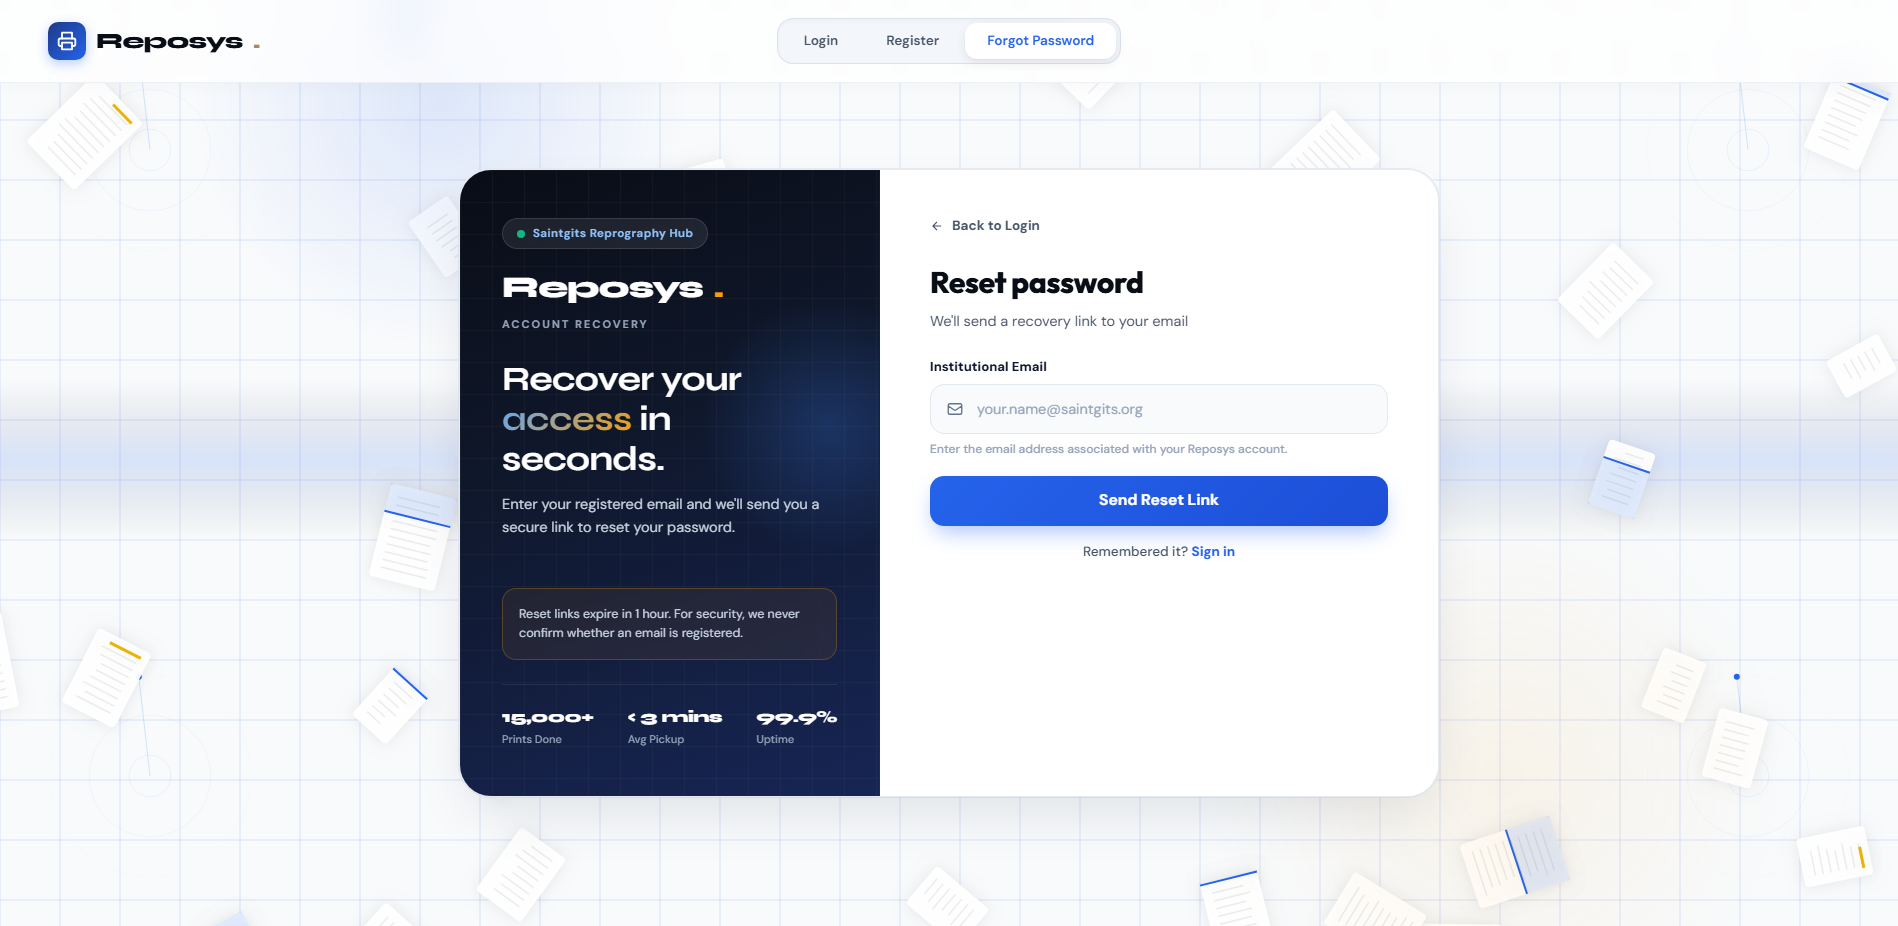
\includegraphics[width=\textwidth,keepaspectratio]{figures/screen_forgot_password.png}
\caption{Account Recovery and Password Reset Workflow}
\label{fig:ui_forgot}
\end{figure}

\begin{figure}[H]
\centering
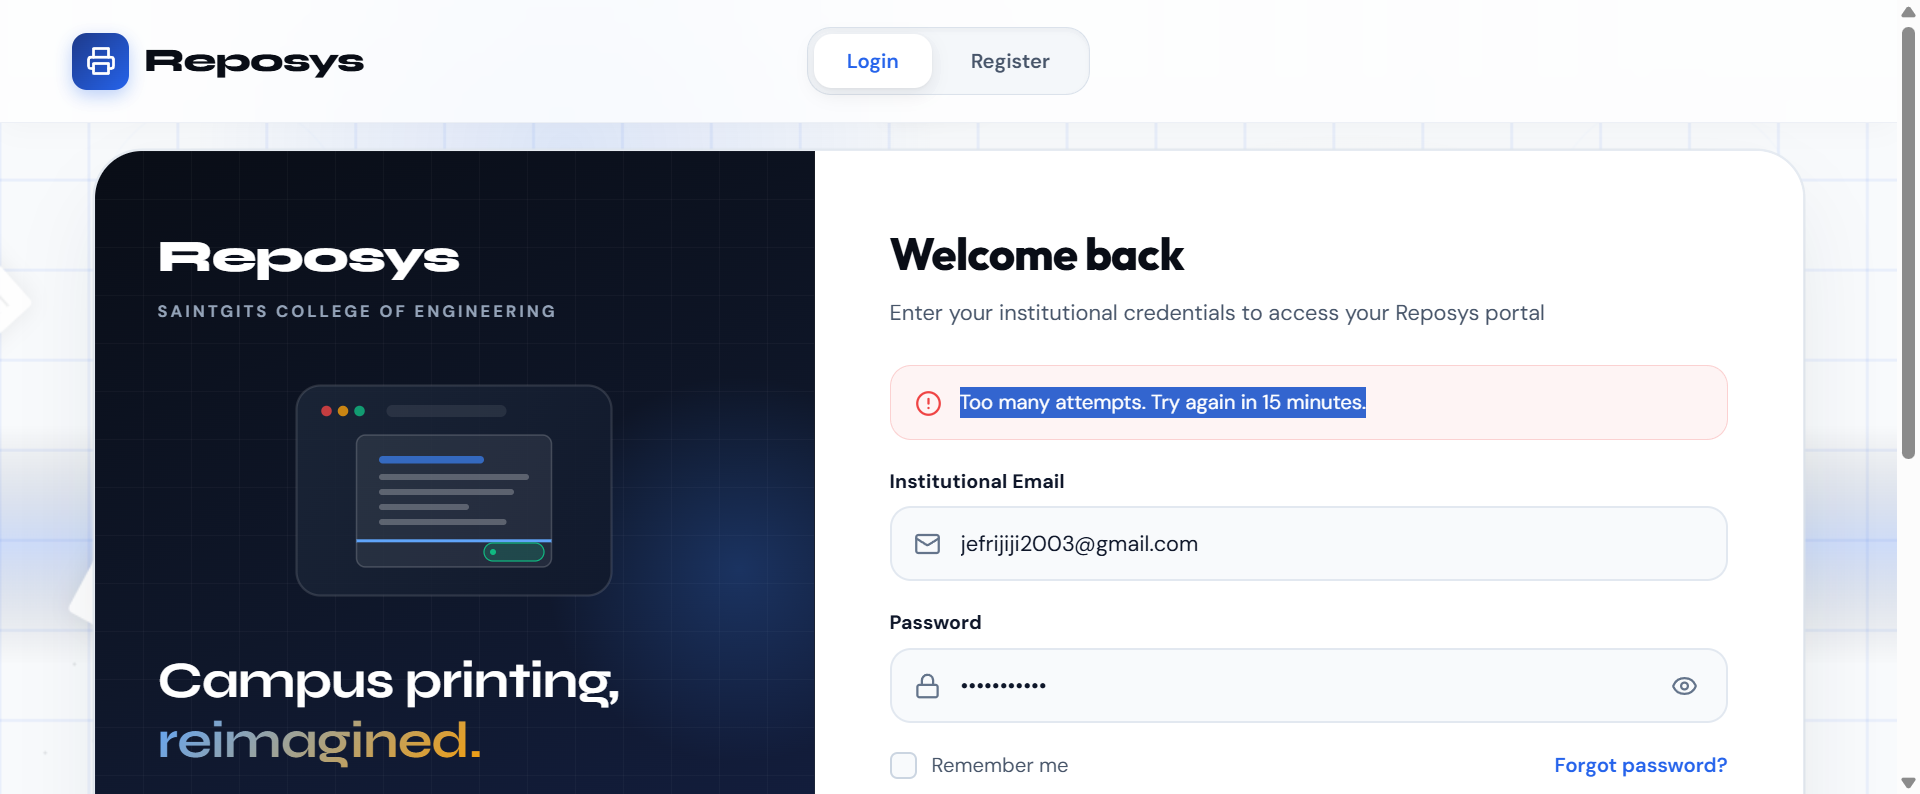
\includegraphics[width=\textwidth,keepaspectratio]{figures/test_student_workflow.png}
\caption{Automated Selenium Test Run: Student Document Upload and Order Creation Workflow}
\label{fig:test_student_workflow}
\end{figure}

\begin{figure}[H]
\centering
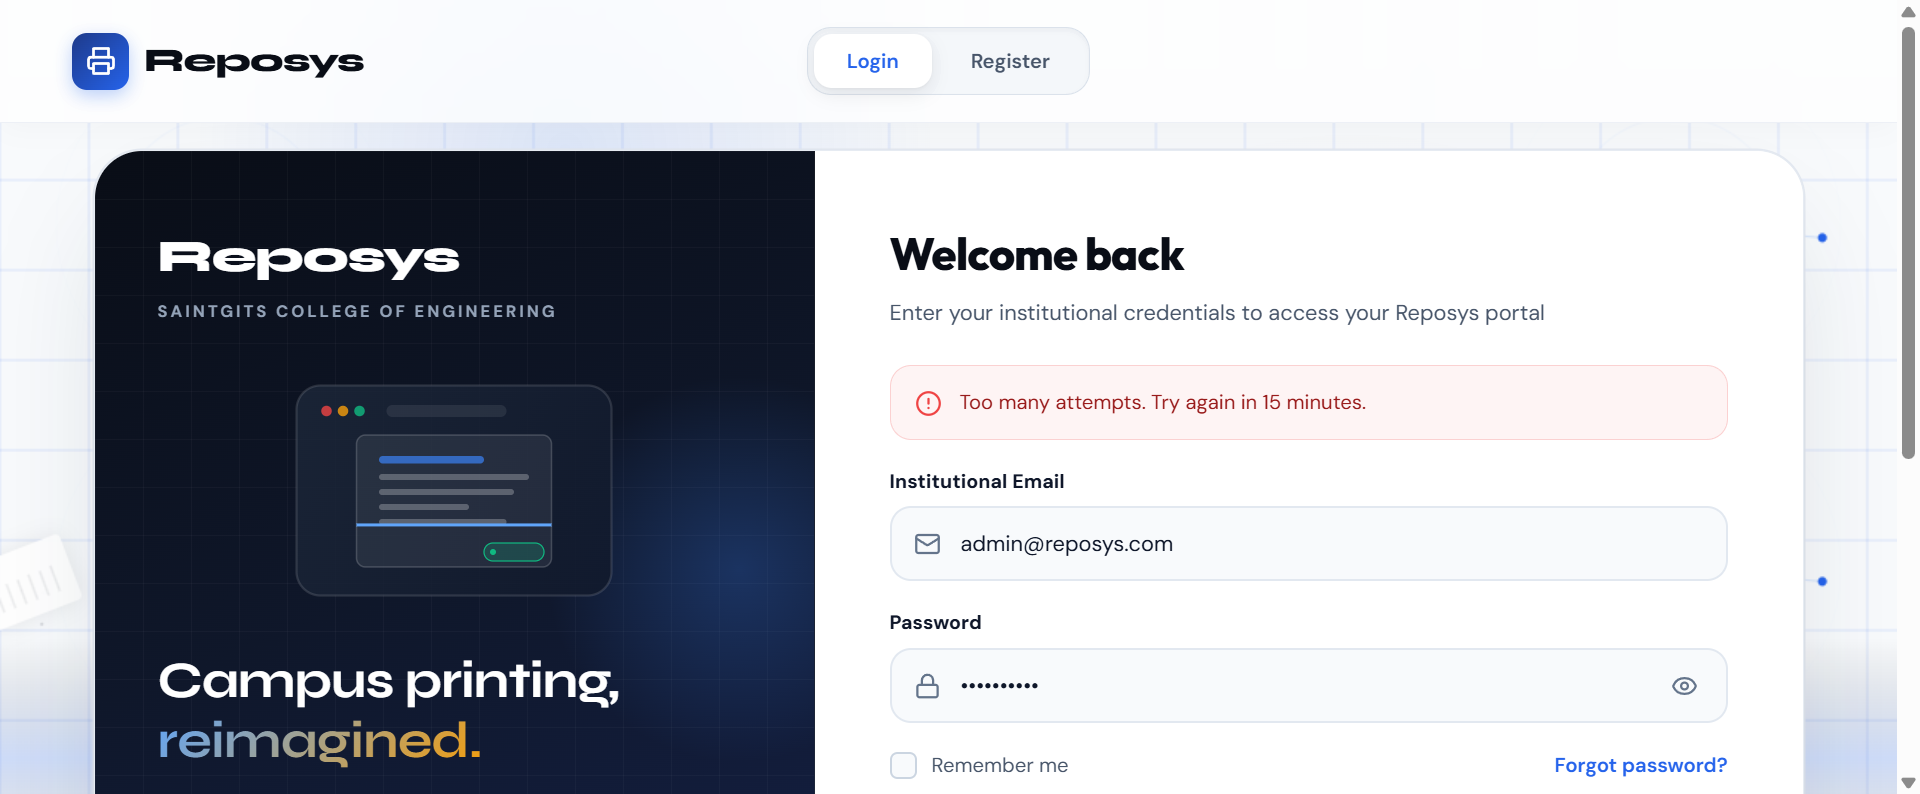
\includegraphics[width=\textwidth,keepaspectratio]{figures/test_admin_access.png}
\caption{Automated Selenium Test Run: Admin Role Route Access and Security Guard Verification}
\label{fig:test_admin_access}
\end{figure}

\begin{figure}[H]
\centering
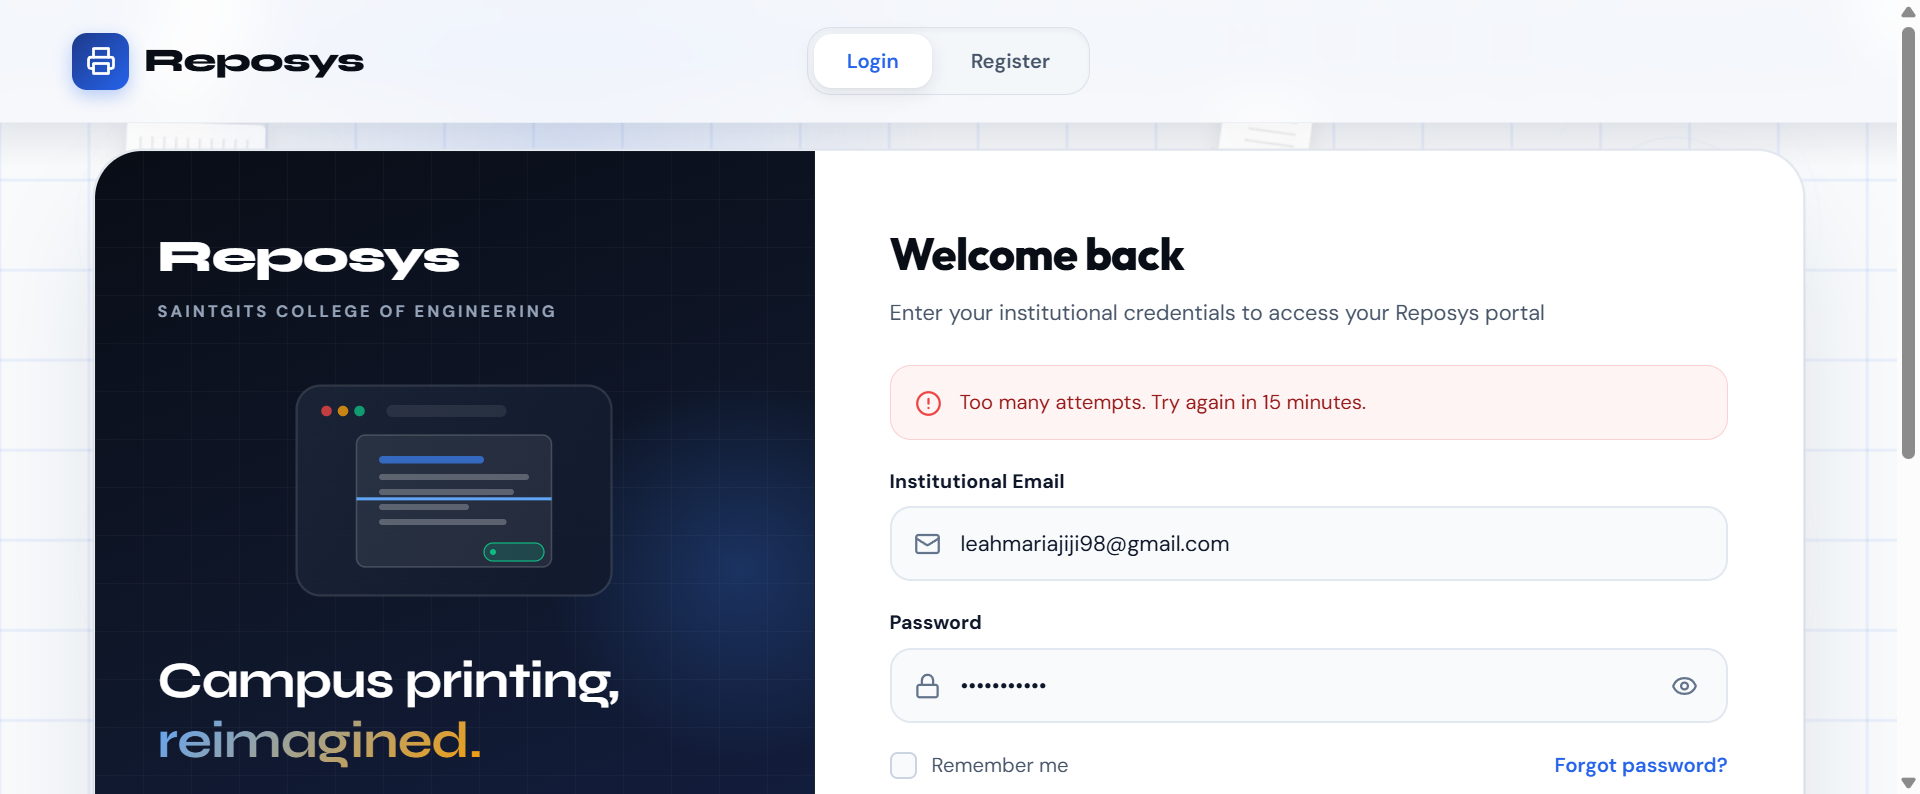
\includegraphics[width=\textwidth,keepaspectratio]{figures/test_staff_access.png}
\caption{Automated Selenium Test Run: Counter Staff Queue Dashboard Access Verification}
\label{fig:test_staff_access}
\end{figure}

\section{8.4 GIT LOGS}
Table 8.1 documents verifiable engineering milestones and commit records extracted directly from the project repository.

\begin{table}[H]
\centering
\small
\begin{tabularx}{\textwidth}{|p{0.75in}|X|}
\hline
\textbf{Commit Hash} & \textbf{Engineering Milestone and Commit Message} \\ \hline
\texttt{5a21841} & fix: synchronize dashboard and profile usage summary \\ \hline
\texttt{04b8040} & update deployment urls for render and vercel \\ \hline
\texttt{510e51a} & update frontend and backend production configurations \\ \hline
\texttt{1a5ce7b} & feat: add TTL to audit logs and Admin Clear All Logs button \\ \hline
\texttt{c0f200e} & feat: remove install settings card, add separate deregister for agents \\ \hline
\texttt{4baffc3} & fix: do not close setup window from main process, let renderer reach step 6 \\ \hline
\texttt{bc077b7} & chore: add comprehensive logging to print agent registration flow \\ \hline
\texttt{fe5c1df} & fix: synchronize print agent socket secret with registration token \\ \hline
\texttt{c9fe161} & fix: replace custom Button with native buttons for ping/deregister \\ \hline
\texttt{c9420b2} & fix: unwrap nested IPC data to prevent agentId/agentSecret undefined \\ \hline
\texttt{ac477ba} & feat: show cold-start wait message during Step 5 registration \\ \hline
\texttt{5882718} & feat: user friendly printer error message during test print setup \\ \hline
\texttt{4fd6368} & fix: extract test.pdf from ASAR archive before printing \\ \hline
\texttt{bd65021} & fix: remove admin installer update instruction and fix token terminology \\ \hline
\texttt{b90df20} & feat: add agent registration verification and live status page \\ \hline
\texttt{7832f82} & feat: add secure print agent download endpoint and admin download card \\ \hline
\texttt{697e8b6} & feat: complete Electron print agent integration and packaging \\ \hline
\texttt{d0596ce} & fix(mobile): Optional chaining for file.name in MobileOrderWizard \\ \hline
\texttt{fbb6d39} & feat: complete SPAE phase 2 print agent integration \\ \hline
\texttt{dbed9a7} & Update PWA mobile screens and UI components \\ \hline
\texttt{0a3ffd3} & fix: remove maskable purpose from PWA icons to prevent text cutoff \\ \hline
\texttt{89bcd22} & feat(pwa): update PWA icons and app name to Reposys \\ \hline
\texttt{cd1cb2e} & chore: final Reposys rebranding and frontend API fallback resolution \\ \hline
\texttt{d286e06} & Fix InventoryManagement crash by importing CardDescription \\ \hline
\texttt{e3118a4} & Update documentation and frontend features \\ \hline
\end{tabularx}
\caption{Verifiable Version Control Commit History (Git Logs)}
\label{tab:git_logs}
\end{table}

% =========================================================================
% CHAPTER 9: REFERENCES
% =========================================================================
\chapter{REFERENCES}

\begin{singlespace}
\begin{enumerate}[leftmargin=0.35in, itemsep=6pt]
  \item APJ Abdul Kalam Technological University. (2020). \textit{Curriculum and Syllabi for Integrated Master of Computer Applications (IMCA) Programme}. KTU Academic Regulations, Thiruvananthapuram, Kerala.
  \item Cloudinary Inc. (2024). \textit{Cloudinary Node.js SDK and Media Management API Documentation}. Retrieved from \url{https://cloudinary.com/documentation}.
  \item Electron Software Foundation. (2024). \textit{Electron Desktop Framework Documentation and Native Node.js Integration Guides}. OpenJS Foundation. Retrieved from \url{https://www.electronjs.org/docs}.
  \item Fielding, R. T. (2000). \textit{Architectural Styles and the Design of Network-based Software Architectures} (Doctoral dissertation). University of California, Irvine.
  \item Fette, I., \& Melnikov, A. (2011). \textit{The WebSocket Protocol}. RFC 6455, Internet Engineering Task Force (IETF).
  \item Gamma, E., Helm, R., Johnson, R., \& Vlissides, J. (1994). \textit{Design Patterns: Elements of Reusable Object-Oriented Software}. Addison-Wesley Professional, Boston.
  \item Google Developers. (2024). \textit{Progressive Web Apps: High Performance Caching and Service Worker Lifecycle}. Google Web Fundamentals. Retrieved from \url{https://web.dev/explore/progressive-web-apps}.
  \item Jones, M., Bradley, J., \& Sakimura, N. (2015). \textit{JSON Web Token (JWT)}. RFC 7519, Internet Engineering Task Force (IETF).
  \item Kleinrock, L. (1975). \textit{Queueing Systems, Volume 1: Theory}. John Wiley \& Sons, New York.
  \item Mozilla Developer Network. (2024). \textit{HTTP Headers, Content Security Policy, and Secure Web API Standards}. MDN Web Docs. Retrieved from \url{https://developer.mozilla.org/}.
  \item Node.js Foundation. (2024). \textit{Node.js v20.x Long Term Support (LTS) API Specification}. OpenJS Foundation. Retrieved from \url{https://nodejs.org/docs}.
  \item Nyberg, K. (2020). \textit{Building Scalable Microservices with Node.js and MongoDB}. O'Reilly Media, Sebastopol.
  \item Pressman, R. S., \& Maxim, B. R. (2020). \textit{Software Engineering: A Practitioner's Approach} (9th ed.). McGraw-Hill Education, New York.
  \item Razorpay Software Private Limited. (2024). \textit{Razorpay Payments API Specification and Webhook Signature Verification Reference}. Retrieved from \url{https://razorpay.com/docs/api}.
  \item React Development Team. (2024). \textit{React 19 Documentation: Server Components, Hooks, and Concurrency Architecture}. Meta Open Source. Retrieved from \url{https://react.dev/}.
  \item Saintgits College of Engineering (Autonomous). (2026). \textit{Department of Computer Applications: Mini Project Preparation Guidelines and Scrum Assessment Manual (20IMCAP501)}. Pathamuttom, Kottayam.
  \item SeleniumHQ. (2024). \textit{Selenium WebDriver Browser Automation Framework Documentation}. Software Freedom Conservancy. Retrieved from \url{https://www.selenium.dev/documentation}.
  \item Socket.IO Foundation. (2024). \textit{Socket.IO Client and Server Bidirectional Event Specification}. Retrieved from \url{https://socket.io/docs/v4/}.
  \item Sommerville, I. (2016). \textit{Software Engineering} (10th ed.). Pearson Education, Harlow, UK.
\end{enumerate}
\end{singlespace}

\end{document}
